\subsection{Deduplication by file types}

\begin{figure} 
	\centering
	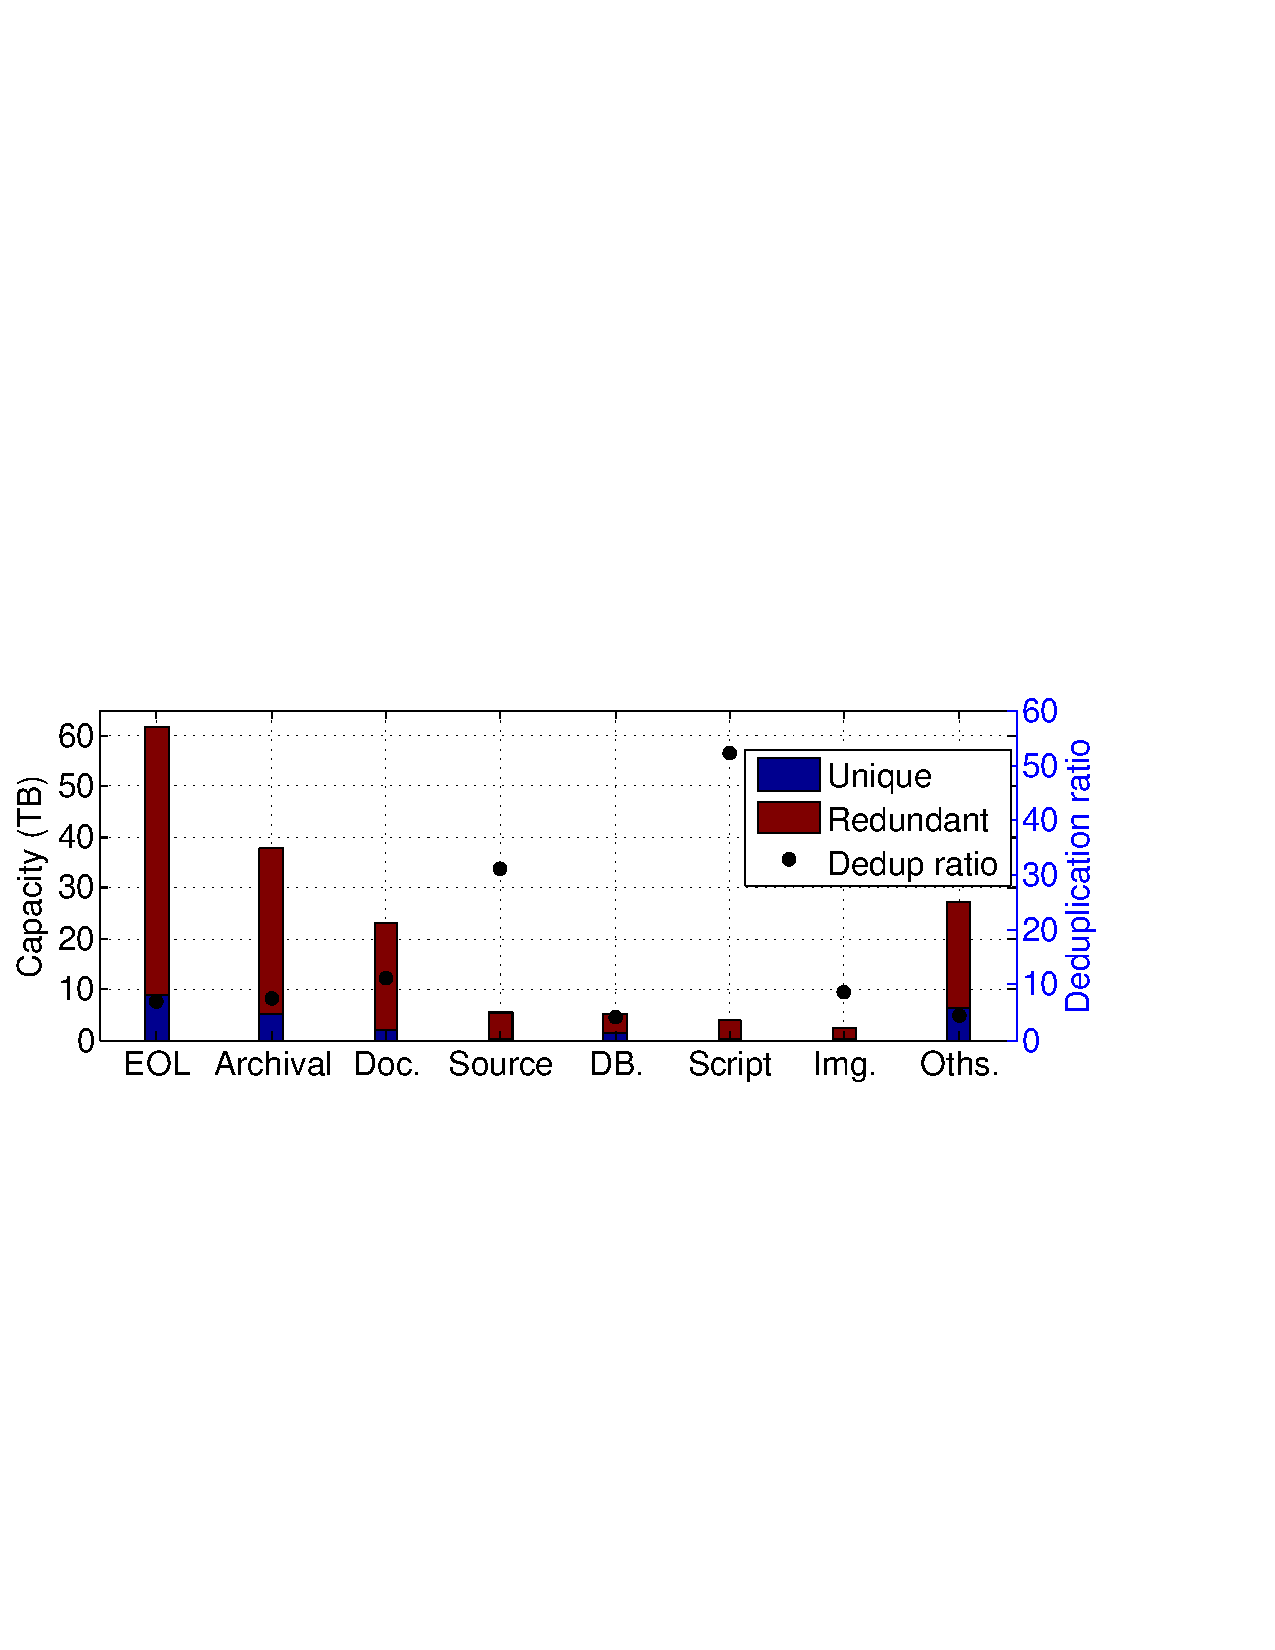
\includegraphics[width=0.45\textwidth]{graphs/dedup-overall} 
	\caption{Deduplication ratio for seven file classes---EOL, archival, documents, source code, database, scripts, images---and other files.
	Light bars indicate the original storage utilization while dark bars represent the capacity after removing redundant files.
	Dots shows the corresponding deduplication ratio.
%
%\VT{Can we stretch X axis to column width to have more space for X-axis labels?}\NZ{addressed}
%%
%\VT{Explain what blue and red bars mean here, as well as dots. Explain
%if dedup ratio is in terms of capacity or file counts.}\NZ{addressed}
%
} 
	\label{fig:dedup-overall} 
\end{figure}




To understand the sources of high data redundancy among Docker images, we
investigate deduplication for common file types.
%
We identify 133 file types (e.g., JPG, C/C++, and Java files)
using the file type library~\cite{pymagic} and then group file types into 7
classes by their high-level use cases:
%
1)~executable, object, and library files (EOL) (such as .o or .pyc)
%
%\VT{Maybe call them ``Exec.`` instead on the graph and everywhere?}
%
2)~archival (such as .gz or .tar),
%
3)~documents (such as .txt or .tex),
%
4)~source code (such as .c or .java),
%
5)~scripts (such as .py or .js),
%
6)~images (such as .png or .eps), and
%
7)~database files (such as .sqlite or .frm). 
%
These classes cover about 88\% of the whole dataset (by capacity);
we group the remaining 12\% in the Others class.
%

Figure~\ref{fig:dedup-overall} illustrates the deduplication results for these
classes.
%
The overall deduplication ratio is \textbf{6.9$\times$} and 4 classes
have a comparable ratio (indicated by the dots).
%
For example, the deduplication ratio for EOL files is \textbf{7.1$\times$}.
%
However, for the other 3 classes, the
deduplication ratio is significantly
higher---\textbf{31.25$\times$} for source code,
\textbf{50$\times$} for scripts, and \textbf{12.5$\times$} for documents.
%
This indicates that users frequently replicate
source code, scripts, and documents in their images.
%
%Moreover, the source code and script duplicates generate additional executables
%and object files that are identical.

We found that redundant C/C++ source code takes up over 77\% of the capacity
occupied by source code files.
%
Looking closer we found that, for example, Google Test~\cite{googletest}---a
cross-platform C++ test framework available on GitHub~\cite{github}---is
frequently replicated.
%
Interestingly, we found there are multiple Docker repositories related to
Google Test but there is no single \emph{official} repository.
%
We think that many developers replicate open source code from external public
repositories, such as GitHub, and store it in container images but do not
specifically encapsulate it in a separate layer. Source code also frequently
changes so if different versions are put into a layer in different images,
a large file base may overlap while few files are different. This can also result
in different layers with high redundancy.
%
%This would also explain the shared source code across different images.
%
%\VT{give few more example in addition ot Google Test}\NZ{addressed}
% 
In addition to Google Test, we also found many replicas of the source code of
go-ethereum~\cite{go-ethereum}, Android Native Development Kit (NDK)~\cite{NDK},
xnu-chroot-environment~\cite{xnu-chroot-environment} among others.
%
%Docker Hub allows developers to automatically build images from
%source code in external public repositories and automatically push the built
%image to their Docker repositories. 
%%https://github.com/ethereum/go-ethereum
%https://github.com/postgres/postgres
%We believe that 
%many developers would replicate
%%more 
%open source codes
%%may be replicated 
%into different images stored in Docker Hub registry.
%
%\VT{I don't understand the last sentence. ``more'' than what?.. And who can 
%replicate? don't use passive voice to make it clear.
%Also, last sentence is too long, please, split.}
%\NZ{commented}
%\VT{not yet ;)}
%
%\textit{To eliminate redundant open source codes in Docker registry in the
%future, we suggest that Docker Hub creates offical images for popular
%open source codebases so developers can directly pull the image as a
%read-only layer}.

Next, we observe that redundant EOL and archival files occupy over half of the
total dataset
capacity (51.4\%). 
%\LR{capacity of what?}\NZ{addressed}.
%
%To understand why there are so many redundant archival files, 
%we manually
%inspected them and found that many archival files contain source codes.
%
%\VT{``many'' is vague}\NZ{addressed}
We analyze the top-5 most frequent archival files.
We found that \texttt{NEWS.Debian.gz}, which stores news
about package changes, has 521,611 copies and
\texttt{pwunconv.8.gz}, which is used to create passwords
has 358,374 copies.
There are two files that have around 87,000 copies:
\texttt{ubuntu\_dists\_trusty\_universe\_Sources.gz} and
\texttt{ubuntu\_dists\_trusty\_universe\_binary-\\amd64\_Packages.gz}, which
contain metadata of the installed packages for the distributions.
%the name, version, size, the description, and the dependencies of the
%installed packages.
%
The last file, \texttt{gcc.log.xz} has 13,384 copies and belongs to the GNU C++ compiler.
%
%For example, we found a highly redundant zip file called
%android-ndk-r12b.zip~\cite{NDK}.
%
%\VT{how many instances of this file were there?}\NZ{addressed}
%
%It packages Android Native Development Kit (NDK) that allows Android
%application developers to include native code in their Android application
%packages, compiled as JNI shared libraries~\cite{NDK}.
%
%\VT{So, Android developers use Docker?..}\NZ{addressed}
% shared-mime-info 24415
%This is mainly because EOL and archival file sizes are bigger than other type
%group.
%
 
%Database related files have the lowest deduplication ratio (\textbf{4.2$\times$}),
%which contributes little to the overall savings.

%All common file types have a high deduplication ratio.  Especially, EOL and
%archival files contribute a lot to the overall savings.
%
%Also, developers are likely to reuse code rather than create their own.
%
%\DIM{Ffrom the data we see there is high source code dedup, but this might be
%too much of a generic statement based on this data.}

%We see that 43.15\% of redundant files are documents, 
%%
%Documents have the
%largest number of redundant files (), indicating that users replicate more
%documents than other clusters. While the redundant document files only consume
%14.54\% (20.87 TB) of storage space, indicating that the size of redundant
%document files are small (10.2 KB on average). In comparison, 13.38\% and
%10.23\% of files are EOL files and source codes, which take up over 3.66\%
%(5.3 TB) and 36.85\% (52.9 TB) of redundant storage space, indicating that
%users replicate source codes and create big identical EOF files (108.6 KB on
%average).
%
%Archival files and scripts have almost similarly number of redundant files,
%8.53\% for archival and 8.69\% for scripts. However, archival cluster consumes
%more storage space than that of scripts (32.9 TB for archival and 3.9 TB for
%scripts) since archival file size (81 KB on avg.) is inherently higher than
%script size (9.4 KB on avg.).
%
%We found that 4.15\% of redundant files are image files and 0.09\% of
%redundant files are relevant to database, which takes 2.1 TB and 3.9 GB
%storage space respectively. There are 10.17\% (21.2 TB) of redundant files in
%\textit{Other} cluster which mainly contains binary data (9.76), GNU message
%catalog (3.37 TB), font related type (3.02 TB), git pack files (1.9 TB), etc. 
%
%\textit{ Finding 1: 13.38\% and 10.23\% of redundant files are source codes
%and EOL files, which take up over 3.66\% (5.3 TB) and 36.85\% (52.9 TB) of
%redundant storage space, indicating that users are more prone to replicate
%source codes and create identical big EOF files, while 43.15\% and 8.53\% of
%redundant files are documents and archival files, which account for 14.54\%
%(20.87 TB) and 22.93\% (32.9 TB) of redundant storage space, indicating users
%replicates more documents and archival files compare to other clusters.}


%
%\begin{figure} 
%	\centering
%	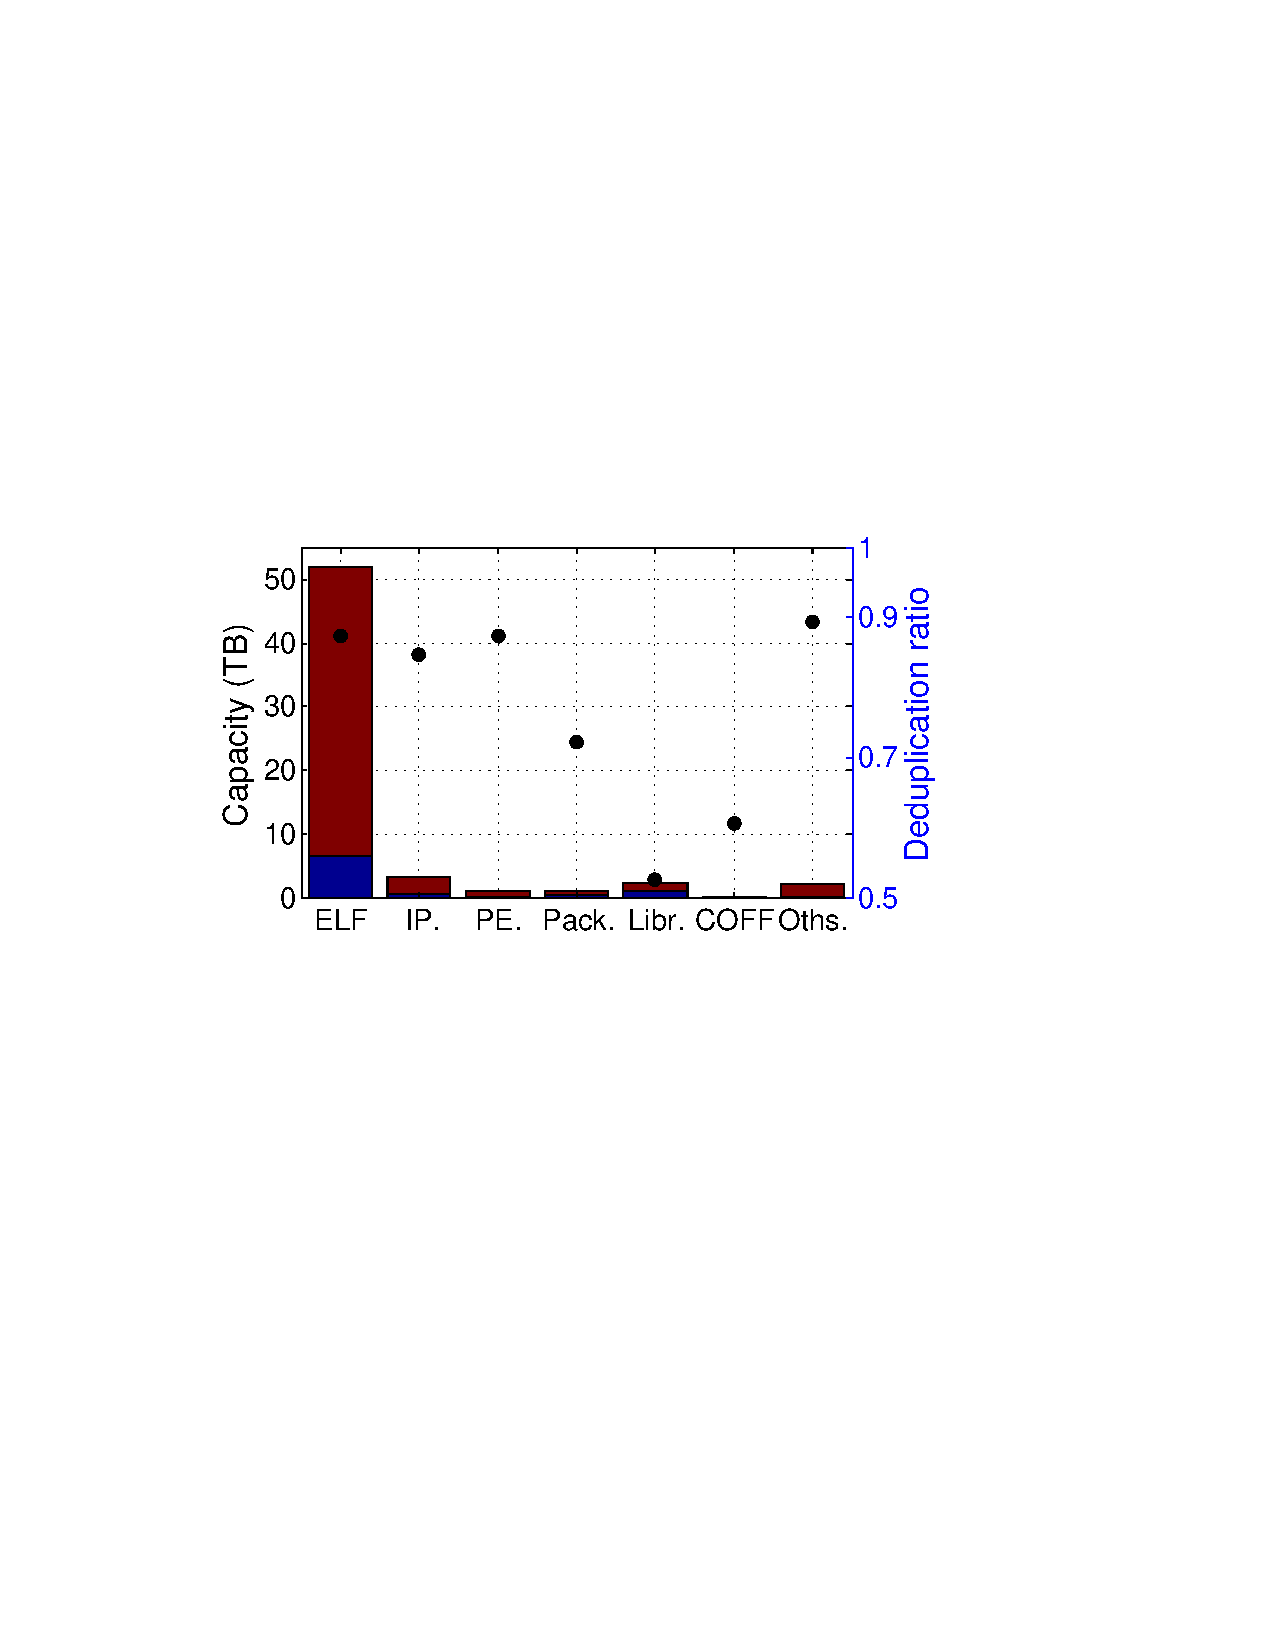
\includegraphics[width=0.35\textwidth]{graphs/dedup-eol} 
%	\caption{Deduplication results for EOL files: ELF, intermediate representation, PE32/PE32+ files, Debian/RPM binary packages, 	Libraries, COFF files.} 
%	\label{fig:dedup-eol}
%\end{figure}
%
%\paragraph{Executable, object code, and libraries (EOL)} We further calculated
%the deduplication ratio for specific file types in each common type group. 
%%
%We
%started from EOL group since it occupies the most capacity and contributes a
%lot to the overall savings after deduplication. 
%%
%Figure~\ref{fig:dedup-eol} shows the deduplication results for EOL files.  
%%
%We
%see that ELF files, intermediate representations, and PE files have the highest
%deduplication ratio (around 87\%). 
%%
%Especially, the redundant ELF files occupy
%the most capacity (73.4\%). 
%%\nancomment{replace MS exec with PE files}
%Libraries and COFF files have the lowest deduplication ratio of 53.5\% and 61\%
%respectively.
%
%We also calculated the deduplication ratio for each intermediate representation
%and libraries. 
%%
%We found that all the intermediate representations have a very
%higher deduplication ratio (greater than 77\%). 
%%
%Especially, the redundant
%Python byte-compiled codes take up to 67\% of capacity occupied by intermediate
%representations. 
%%
%Although overall library's deduplication is lower, we found
%that GUN C/C++ library and Palm OS dynamic library have a higher deduplication
%ratio over 90\%.
%
%\textit{Finding 4: ELF files have the highest deduplication ratio among all EOL
%files and contribute most to the overall savings. Python byte-compiled codes
%have the highest deduplication ratio and also achieve a better capacity savings
%after dedupliation compared with other intermediate representations. Most
%libraries have the lowest deduplication ratio among all EOL files.}
%%
%%%As shown in , intermediate compiled files have the largest number of
%%redundant copies (333,261,220, 63.7\%), which only take up to 5.3\% (2.8TB) of
%%EOL redundant storage space, indicating that users creates more small
%%redundant intermediate compiled files. Among all the intermediate compiled
%%files, python byte-compiled files have the largest number of redundant copies
%%(64.1\%, 213,753,591), which account for 79.4\% (2.2TB) of EOL redundant
%%storage space as shown in Figure~\ref{fig:type-compiled}.  % %We found that
%%there are various redundant intermediate compiled files in layers in addition
%%to Python byte-compiled, such as Erlang beam files, Xemacs/emacs compiled
%%files, compiled Java class, Mach-o fat files, Guile object bytecode, and llvm
%%bitcode files. We see that 21.6\% (71,830,155) and 10.12\% (33,740,399) of
%%redundant intermediate compiled files are terminfo compiled and compiled java
%%class files, which consume 76.4 GB and 104.4 GB storage space.   
%%
%%%ELF files have the largest redundant capacity %A large executable group is
%%ELF file type, which consists of ELF 64/32-bit LSB relocatable, shared object,
%%executable, core file, processor-specific for x86-64, MIPS, %ARM, Intel 80386,
%%etc. architectures.  %Another executable group contains VAX COFF executable,
%%PE32/PE32+ executable for Windows, and 386 pure executable, VMS Alpha, etc.
%%%\% of files are script executable, which contains python, shell, etc.  %\% of
%%files are RPM, Debian bin
%%
%%%\begin{figure} %	\centering %
%%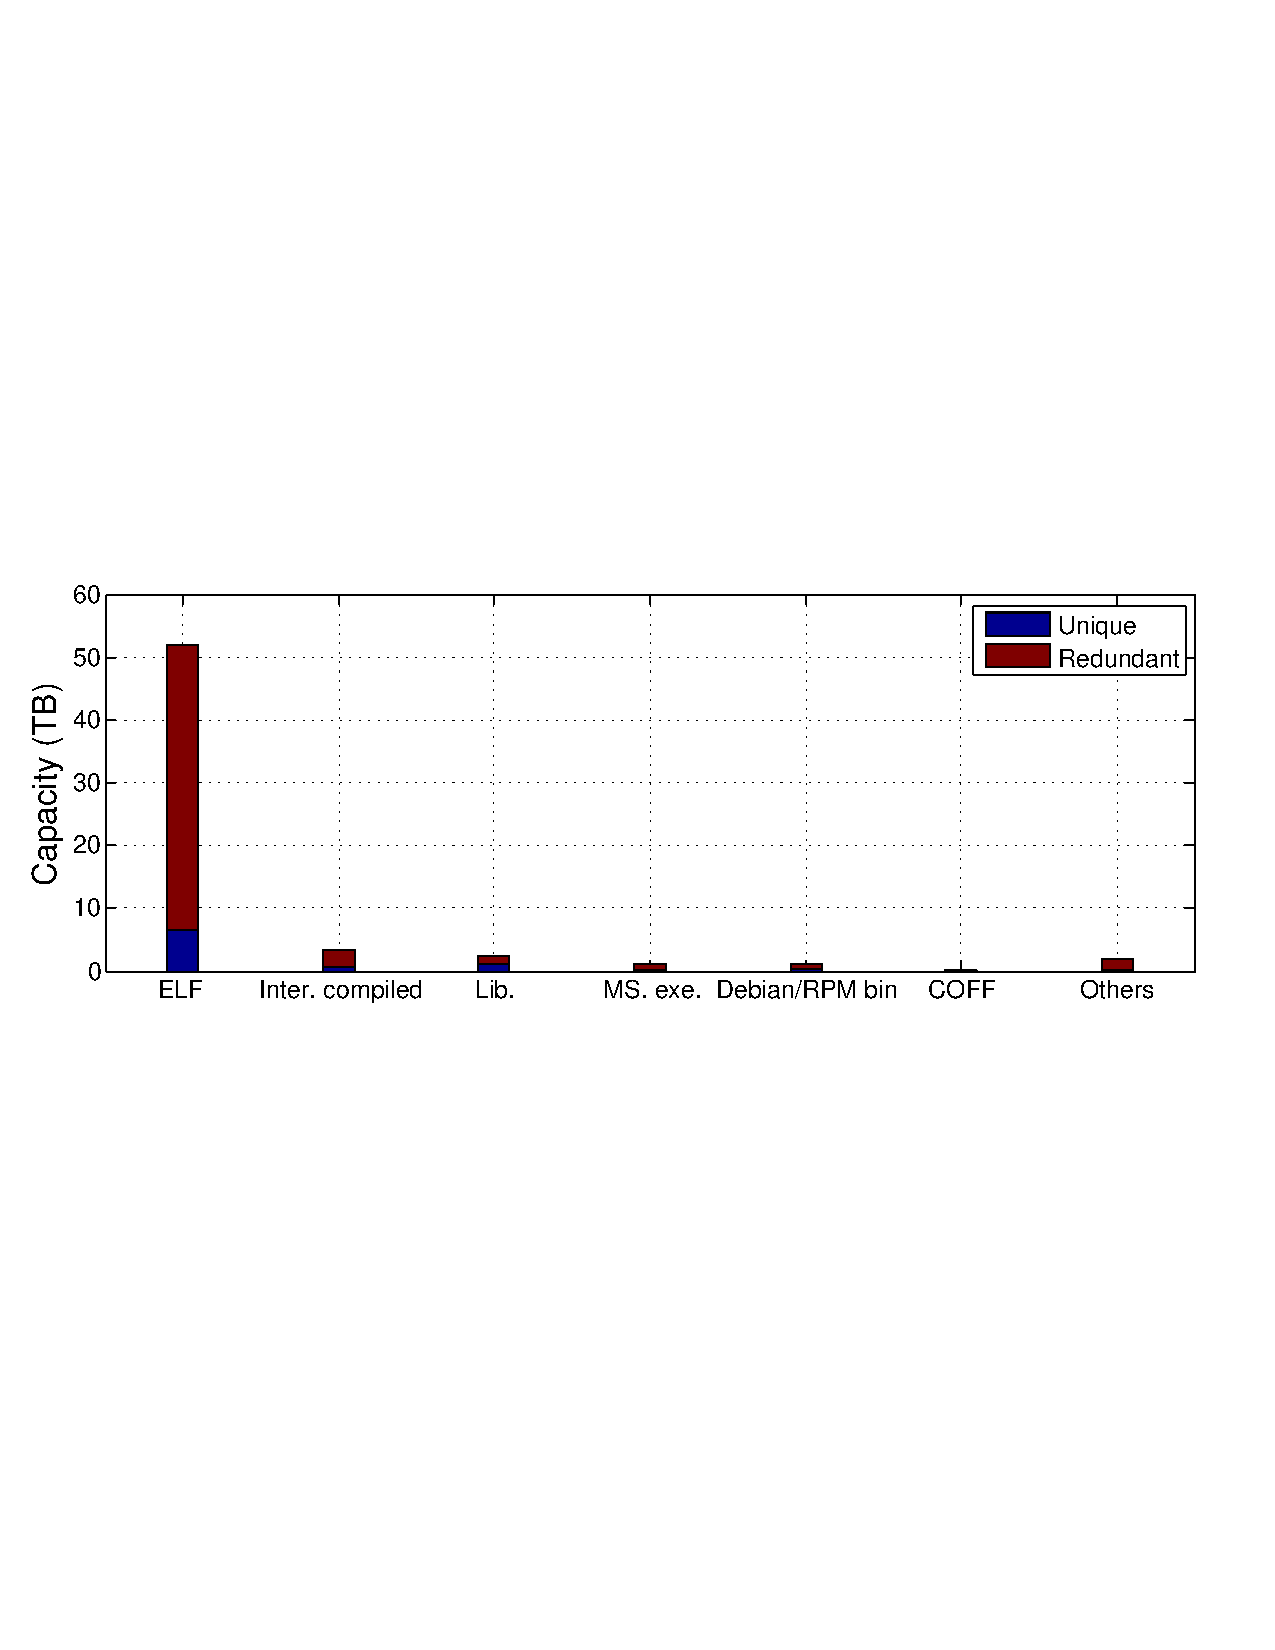
\includegraphics[width=0.5\textwidth]{graphs/type-exec-cap} %
%%\caption{\nancomment{Deduplication results for EOL files}.  %	} %
%%\label{fig:type-eol} %\end{figure}
%%
%%%Finding 2: 31.4\% (164,059,690) and 63.7\% (333,261,220) of EOL files are ELF
%%files and intermediate compiled files, which take up over 85.7\% (45.3TB) and
%%5.3\% (2.8TB) of redundant storage capacity, indicating that users replicate
%%or create more identical ELF files and intermediate compiled files. 64.1\%
%%(213,753,591) of intermediate compiled files are Python byte-compiled files,
%%which take up to 79.4\% (2.2TB) of redundant storage space, indicating that
%%users compiled more Python scripts (similar to Finding 2.)
%%
%\paragraph{Source code (SC.)}
%%
%%%Finding 3: 80.2\% (548,507,865) of source codes are C/C++ source, which take
%%up to 79.7\% (4.2TB) of redundant storage space, indicating that users are
%%more prone to duplicate C/C++ codes, which results in more ELF file replicas.
%%%The last group contains
%%
%\begin{figure} 
%	\centering
%	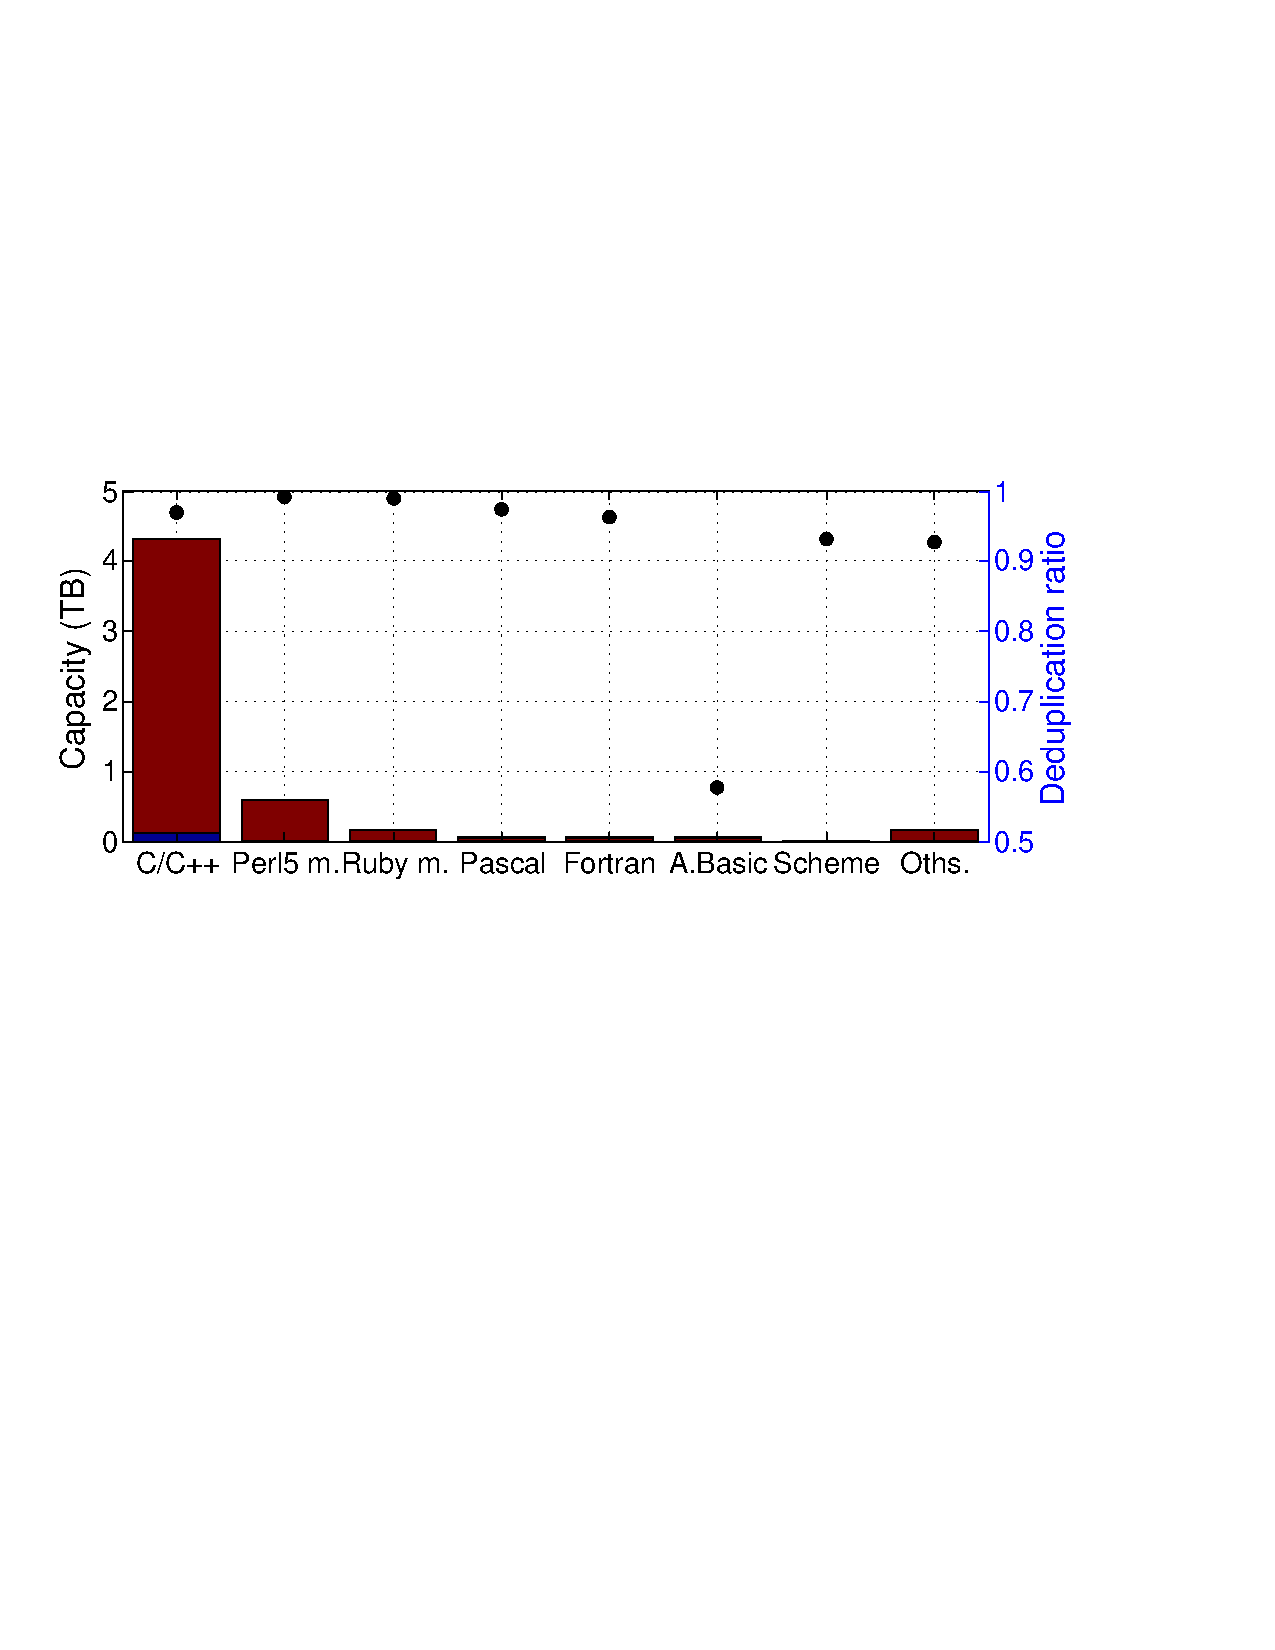
\includegraphics[width=0.35\textwidth]{graphs/dedup-sc} 
%	\caption{Deduplication results for source codes: C/C++ source, Perl5 module source, ruby module
%		source, pascal program, fortran program, Applesoft Basic program, Lisp/scheme
%		program, and other source codes.  } 
%	\label{fig:dedup-sc} 
%\end{figure}
%
%As discussed, Docker developers are more prone to replicate codes. 
%%
%To find out
%which kind of source codes are replicated frequently, we conducted
%deduplication on 7 common source codes as shown in Figure~\ref{fig:dedup-sc}.
%
%We see that all the source codes have a high deduplication ratio over 90\%
%except Lisp/scheme program. 
%%
%Especially, the redundant C/C++ source codes take
%up over 77\% of capacity occupied by source codes. 
%%
%To find out why there are so
%many C/C++ source codes, we inspect the C/C++ source codes and find a
%frequently replicated C/C++ source code called Google Test~\cite{googletest}, which is
%a cross-platform C++ test framework and available in GitHub~\cite{github}.
%%
%Interestingly, we found there are plenty of repositories related to Google Test
%while there is no official repository for Google Test. 
%%
%We suspect that many
%developers replicate open source code from external public repositories, such
%as GitHub, and store them in containers. 
%%
%This would also explain why there are
%so many shared source codes across different images. 
%%
%Docker Hub
%allows developer to automatically build images from source code in external
%public repositories and automatically push the built image to their Docker
%repositories. Thus we believe that more open source code would be replicated into
%different images stored in Docker Hub registry. 
%%
%\textit{To eliminate redundant
%open source codes in Docker registry in the future, we suggest that Docker Hub
%can create more offical images for popular open source codes so that developers
%can directly pull the image as a read-only layer. }
%
%\textit{Finding 5: C/C++ source codes have a high redundant ratio and
%contribute a lot to the overall savings. Many redundant source codes shared
%cross images are replicated or automatically build from external public
%repositories. To eliminate redundant source codes in Docker registry, we
%suggest to create more official images for these open source codes and convince
%developers to pull them from registry.}
%%
%%%\nancomment{found some libc++ source code here, did not put them into
%%libraries.} % shows the redundant file count and storage capacity distribution
%%for source code. C/C++ source codes have the largest number of redundant
%%files. 80.2\% (548,507,865) of source codes are C/C++ source, which take up to
%%79.7\% (4.2TB) of redundant storage space, indicating that users are more
%%prone to duplicate C/C++ codes, which results in more ELF file replicas.
%%
%%%We also found other source codes, such as Perl5 module source code (9.5\%),
%%ruby module source code (7.6\%), assembler source code (1.1\%), pascal source
%%(0.7\%), fortran program code (0.01\%), applesoft basic source code, and
%%Lisp/scheme source code (0.17\%).
%%
%%%\begin{figure} %	\centering %
%%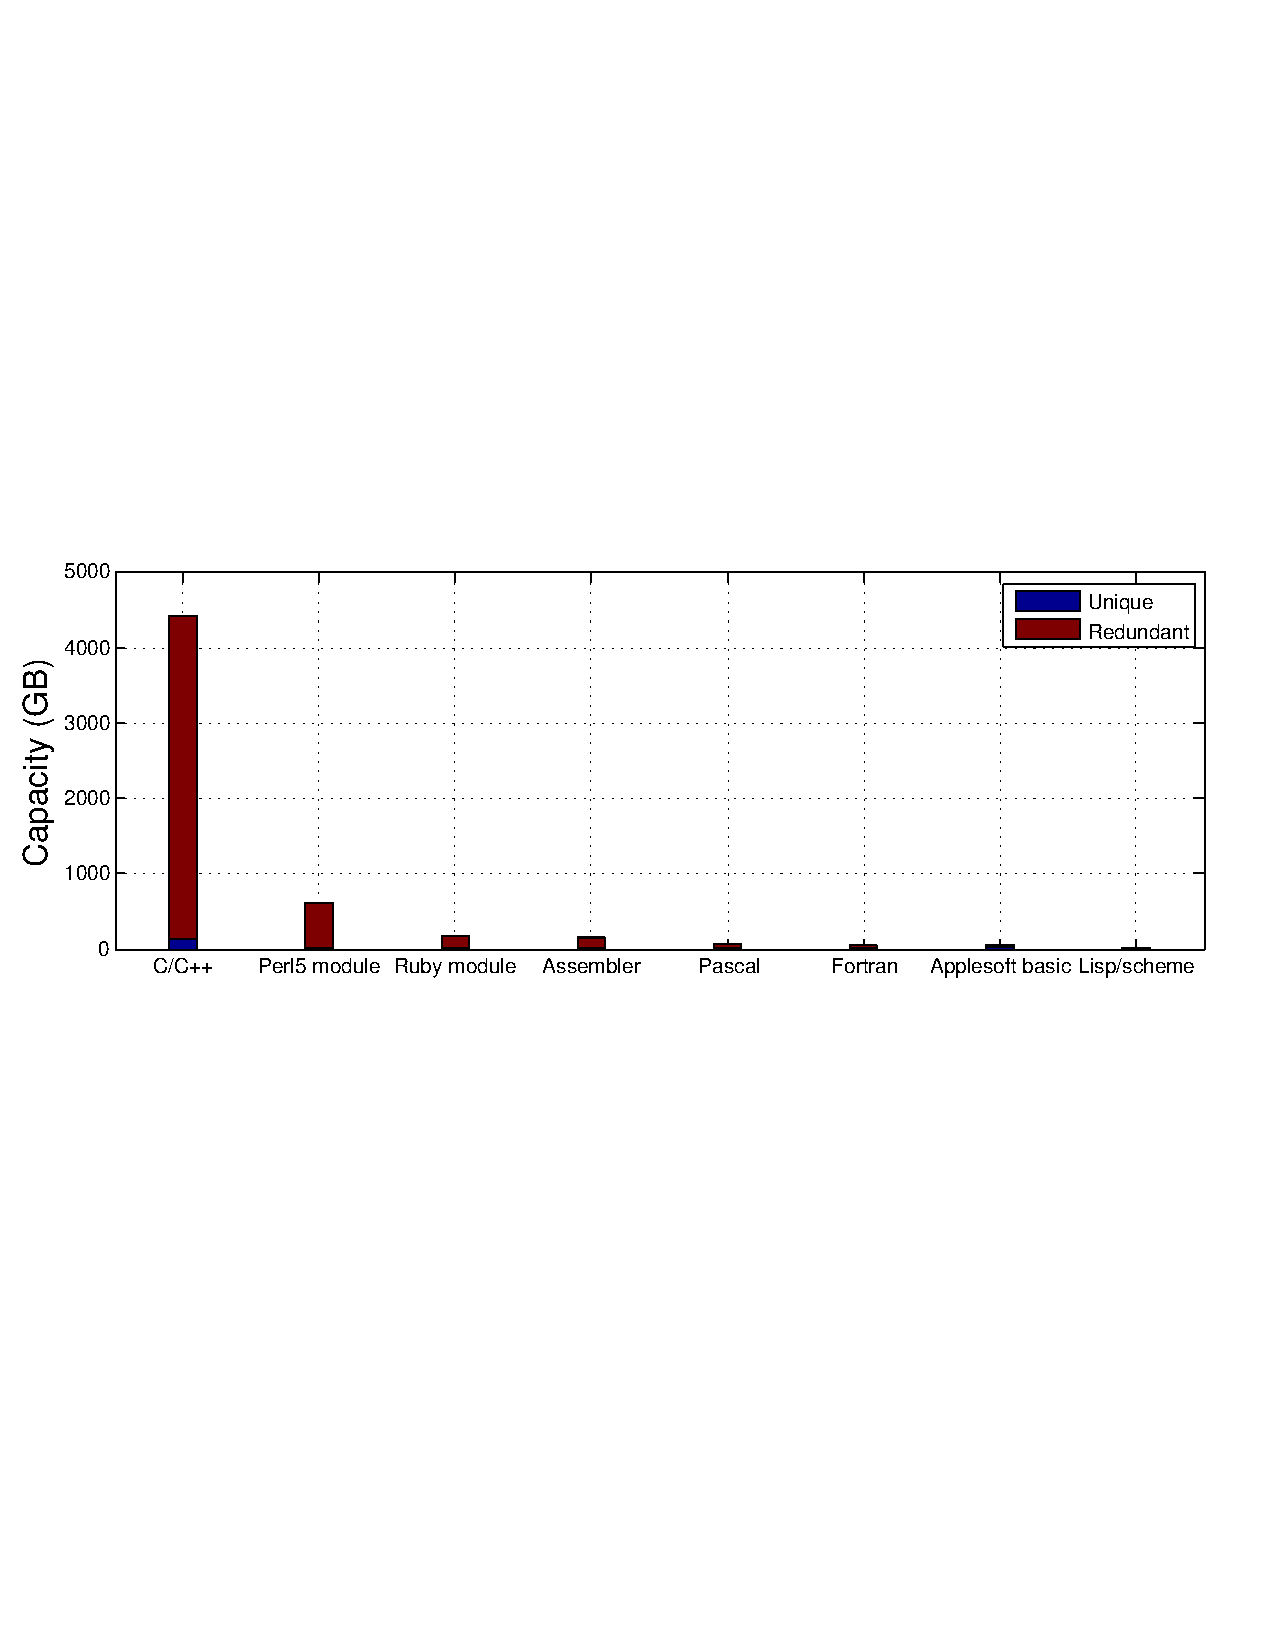
\includegraphics[width=0.5\textwidth]{graphs/type-lang-cap} %
%%\caption{Redundant data vs. unique data for source code files.  %	} %
%%\label{fig:type-source} %\end{figure}
%%
%%%Figure~\ref{fig:type-lib} shows the redundant library distribution. We see
%%that Gcc precompiled header files have the lowest number of redundant library
%%files (20.3\%), but they take up to 0.93 TB. Almost 86.4\% of redundant
%%library files are Palm libraries, which only take up to 7.2GB space,
%%indicating that gcc compiled header files are much bigger than other
%%libraries.  % %We also found there are different libraries used in layers,
%%such as netcdf library, Ocaml lib., mach-o lib.
%%
%%%Figure~\ref{fig-elf} %\subsection{Lib} % %library files contains libtool
%%library file, OCaml native library, MIT scheme, Mach-O library, OCaml library,
%%Palm OS dynamic library data, Microsoft c/c++ library.current ar archive
%%random library, and other library.
%%%%libtool\|OCaml\|Palm\|MIT\|microsoft\|current ar archive random
%%library\|mach-o\|rpm\|gzip %\subsection{Source code}
%%
%\paragraph{Scripts(Scr.)}
%%%Finding 2: 53.6\% (238,353,674) of redundant scripts are Python scripts,
%%which take up over 2.6TB storage space, indicating that users are more prone
%%to replicate Python scripts compare to other scripts.
%%
%%%\begin{figure} %	\centering %
%%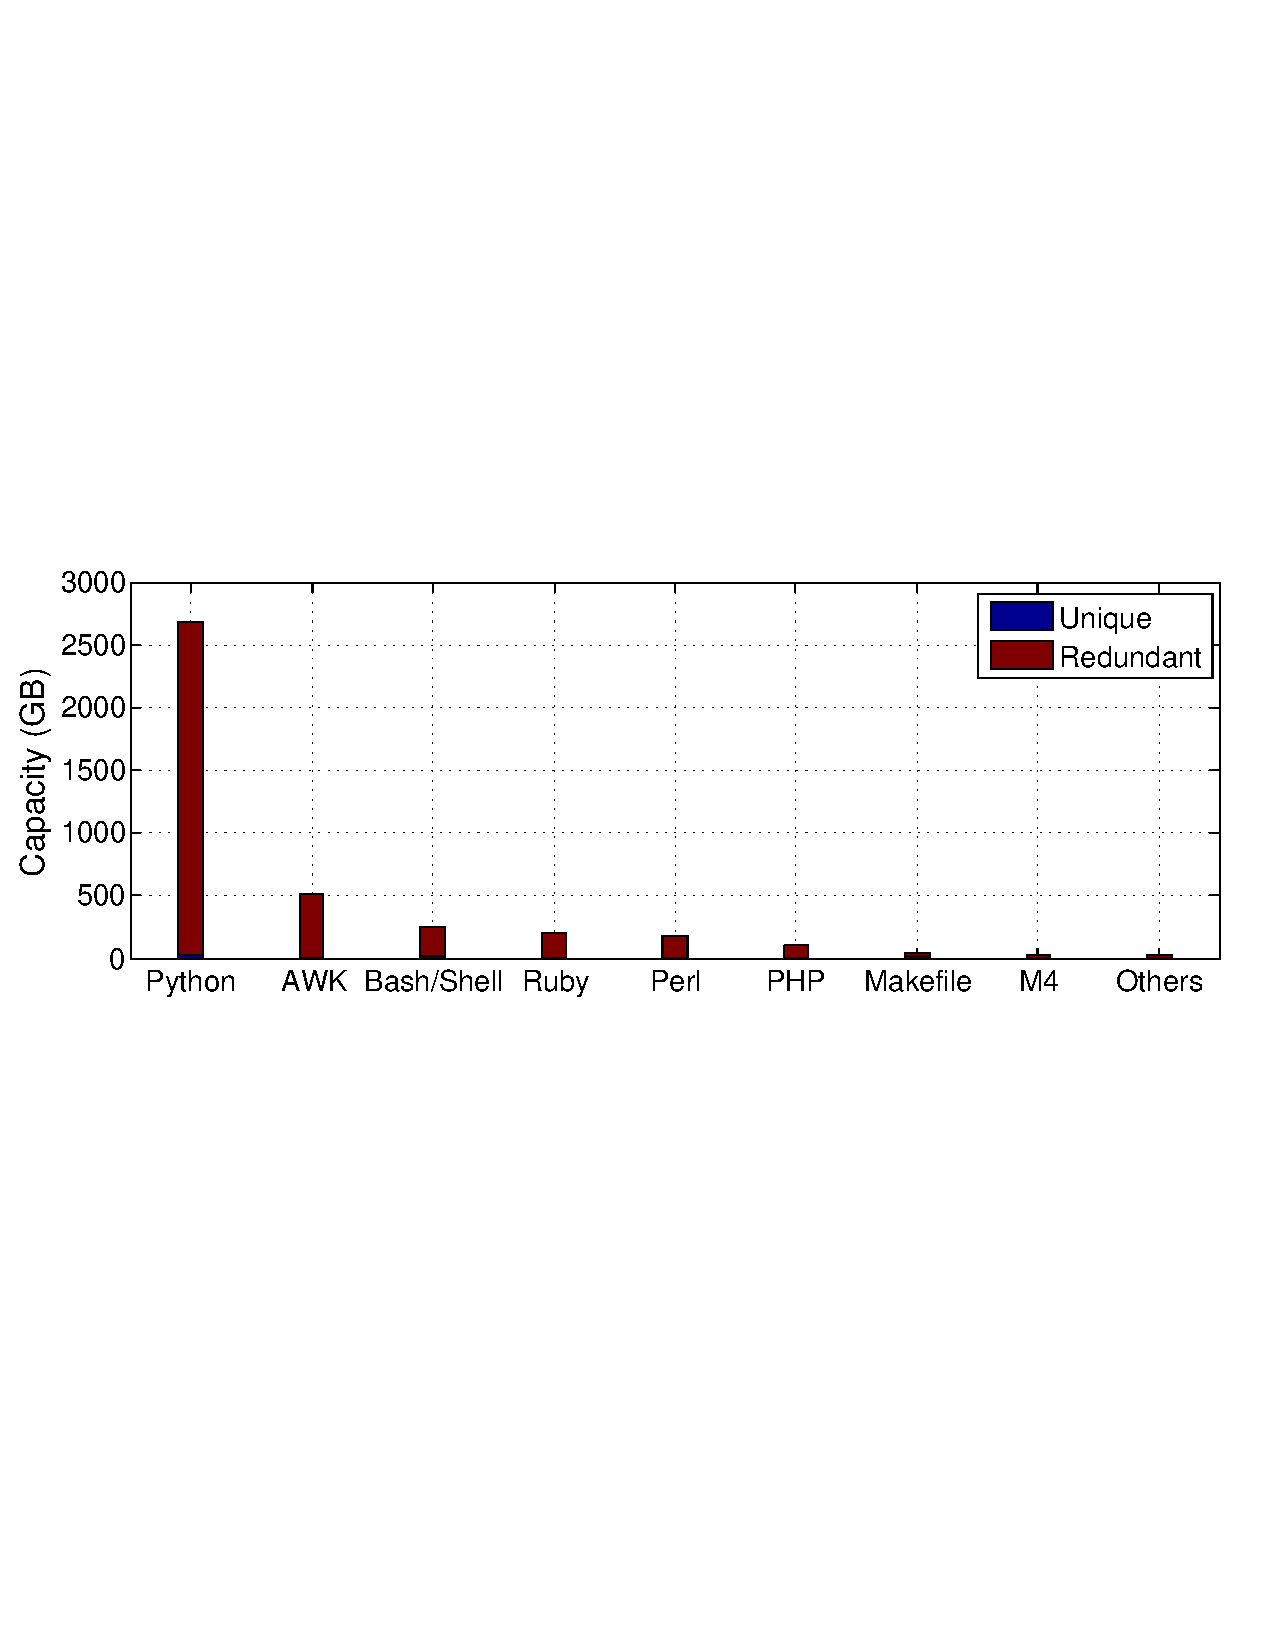
\includegraphics[width=0.5\textwidth]{graphs/type-script-cap} %
%%\caption{Redundant data vs. unique data for scripts.  %	} %
%%\label{fig:type-script} %\end{figure}
%%
%
%\begin{figure} 
%	\centering
%	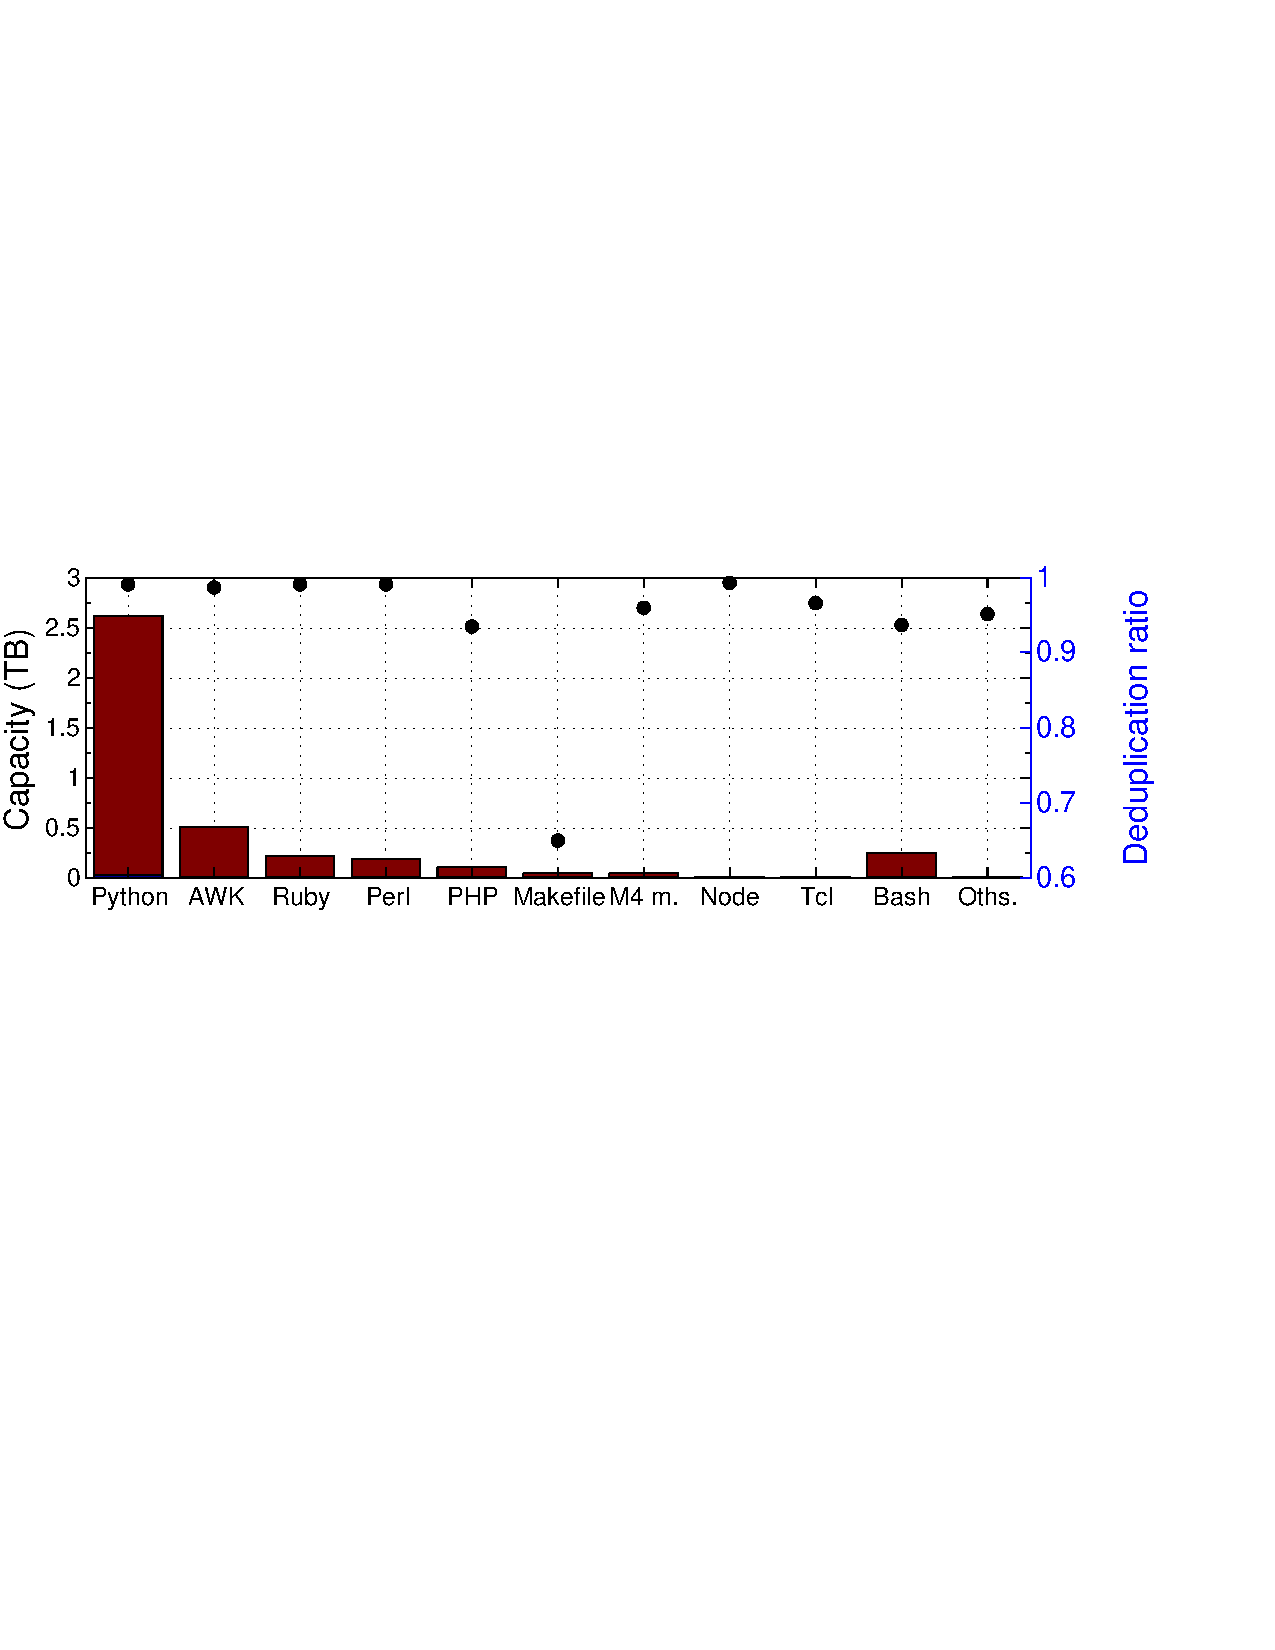
\includegraphics[width=0.45\textwidth]{graphs/dedup-scrp}
%	\caption{Deduplication results for scripts: python, AWK, ruby, perl, PHP, makefile, M4 macro processor, node, Tcl, bash and other scripts.}
%	\label{fig:dedup-scrp} 
%\end{figure}
%
%Similar to source codes, we present the deduplication ratio for scripts as
%shown in Figure~\ref{fig:dedup-scrp}.  
%%
%We see that most of the scripts have a
%high deduplication ratio over 95\%. 
%%
%Especially, the redundant Python scripts
%take up over 65\% of capacity occupied by scripts. 
%
%We inspect the Python scripts and found a frequently replicated Python scripts
%called kraken-tools~\cite{krakentools}, which is a tool for managing system
%requirements for kraken-lib~\cite{krakenlib}. 
%%
%kraken-lib is an orchestration and
%cluster-level management system for Kubernetes~\cite{kubernetes}.
%%% a tool for  for Kubernetes cluster.  %kraken-lib %Kubernetes is an open
%%source platform that automates Linux container operations 
%%
%Although kraken-tools seems like an Docker image repository, it is maintained
%in GitHub rather than Docker registry. 
%%
%Interestingly, kraken-lib does not have
%a official repository in Docker Hub but it has a public repository in QUAY
%registry~\cite{quay}.  
%%
%\textit{Similar to source codes, we suggest to create
%more official images in registry for some popular public scripts %, especially
%containerized applications and convince developers to pull them from registry
%as a read-only layer to reduce redundant scripts in registry.}
%
%\textit{Finding 6: Scripts have a very high deduplication ratio. Especially,
%redundant Python scripts contribute a lot to the overall savings. Many
%redundant scripts are replicated from external public repositories such as
%GitHub.  we suggest to create more official images for these public scripts and
%convince developers to pull them from registry.}
%%% shows the redundant scripts distribution. Python script has the largest
%%number of redundant scripts (238353674, 53.6\%), which take up to 2.6TB
%%storage space, indicating that users are more prone to replicate Python
%%scripts compare to other scripts.  %%This finding also explains that why
%%python byte compiled files takes the largest proportion of intermediate % %We
%%find that users use different scripts in the images.  %For example, 20\%,
%%9.7\% and 4.4\% of scripts are bash/shell scripts, ruby scripts, and awk
%%scripts. Other scripts such as perl script (4.2\%), php script(3.9\%),
%%makefile script(1.3\%), and M4 macro processor script(0.7\%) are also used.
%%
%\paragraph{Documents(Doc.)}
%%%Finding 3: 79.7\%, 5.2\%, and 12.4\% of redundant documents are ASCII text,
%%UTF-8/16 text, and HTML/XML/XHTML, which take up over 11TB, 3.4TB, and 3.9TB
%%redundant storage, indicating that users replicate more ASCII text, UTF-8/16
%%text, and HTML/XML/XHTML compare to other documents.
%%
%\begin{figure} 
%	\centering
%	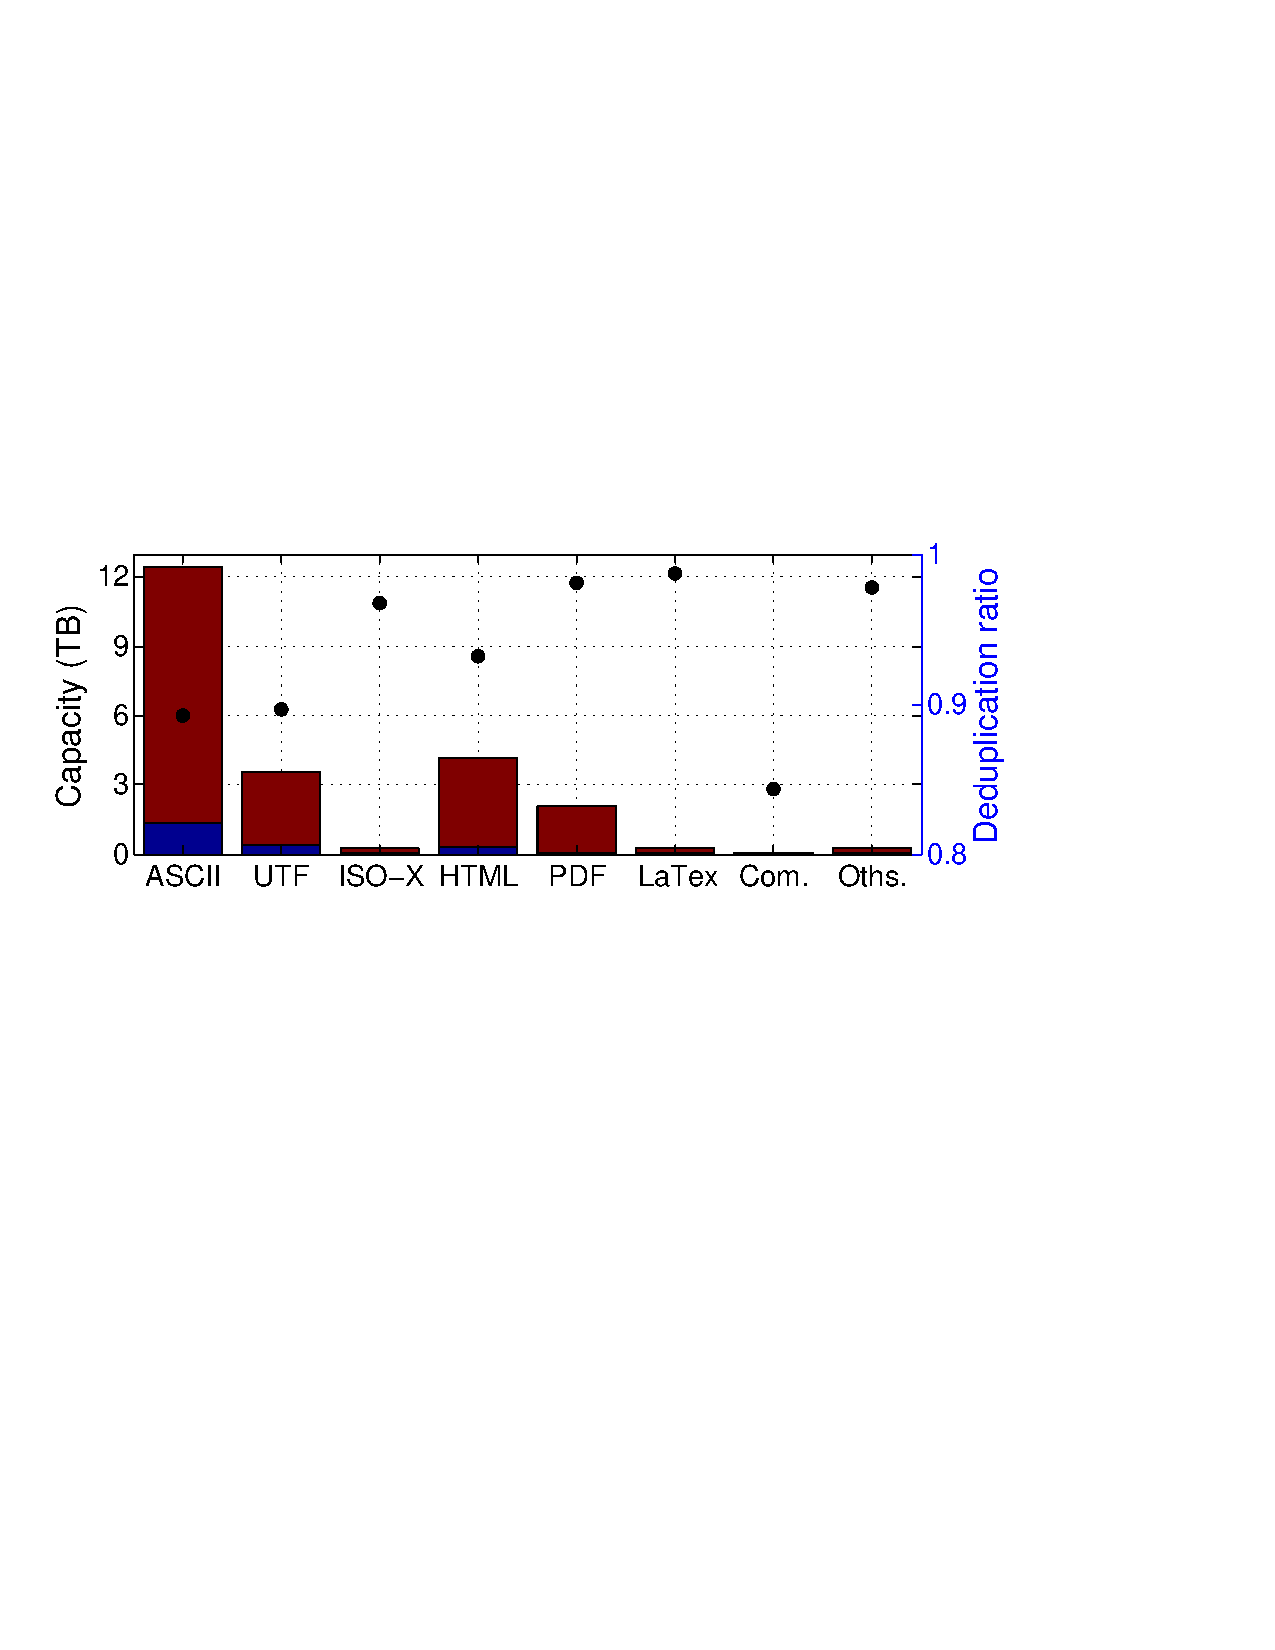
\includegraphics[width=0.35\textwidth]{graphs/dedup-doc} \caption{Deduplication
%	results for documents: ASCII, UTF, ISO-8859, HTML/XML/XHTML, PDF, LaTex
%	documents, Composite document files, and others.} 
%	\label{fig:dedup-doc}
%\end{figure}
%
%Next, we present the deduplication results for different documents as shown in
%Figure~\ref{fig:dedup-doc}.  
%%
%We see that all the documents have a very high
%deduplication ratio of 84\% or higher.  
%%
%Especially, redundant raw text files
%and HTML/XML/XHTML documents take up over 48\% and 17\% of capacity occupied by
%documents. 
%%
%To understand why there are so many document duplicates, we inspect
%raw text files and HTML/XML/XHTML documents respectively. 
%%
%First, we found that
%a large amount of redundant raw text files are input data for testing source
%codes and they are replicated along with source code or script projects from
%external public repositories.  
%%
%For example, scipy~\cite{scipy}, a
%metamathematical software, is replicated from GitHub and stored in different
%images, which contains over 30 raw text files for testing purpose.
%
%Second, after inspected HTML/XML/XHTML documents, we found plenty
%HTML/XML/XHTML documents serves as readme, manual, or license. 
%%
%For example, we
%found plenty redundant HTML documents related to gnome-vfs-doc~\cite{gnome-vfs-doc},
%which are documentation for GNOME virtual filesystem subsystem available
%online~\cite{gvfs}.
%
%\textit{Finding 7: Documents have a very high redundant ratio. Majority
%redundant documents are raw text files and HTML/XML/XHTML documents. They are
%replicated along with source code or script projects and serves as input data
%for testing or informative documents.}
%%
%%%\begin{figure} %	\centering %
%%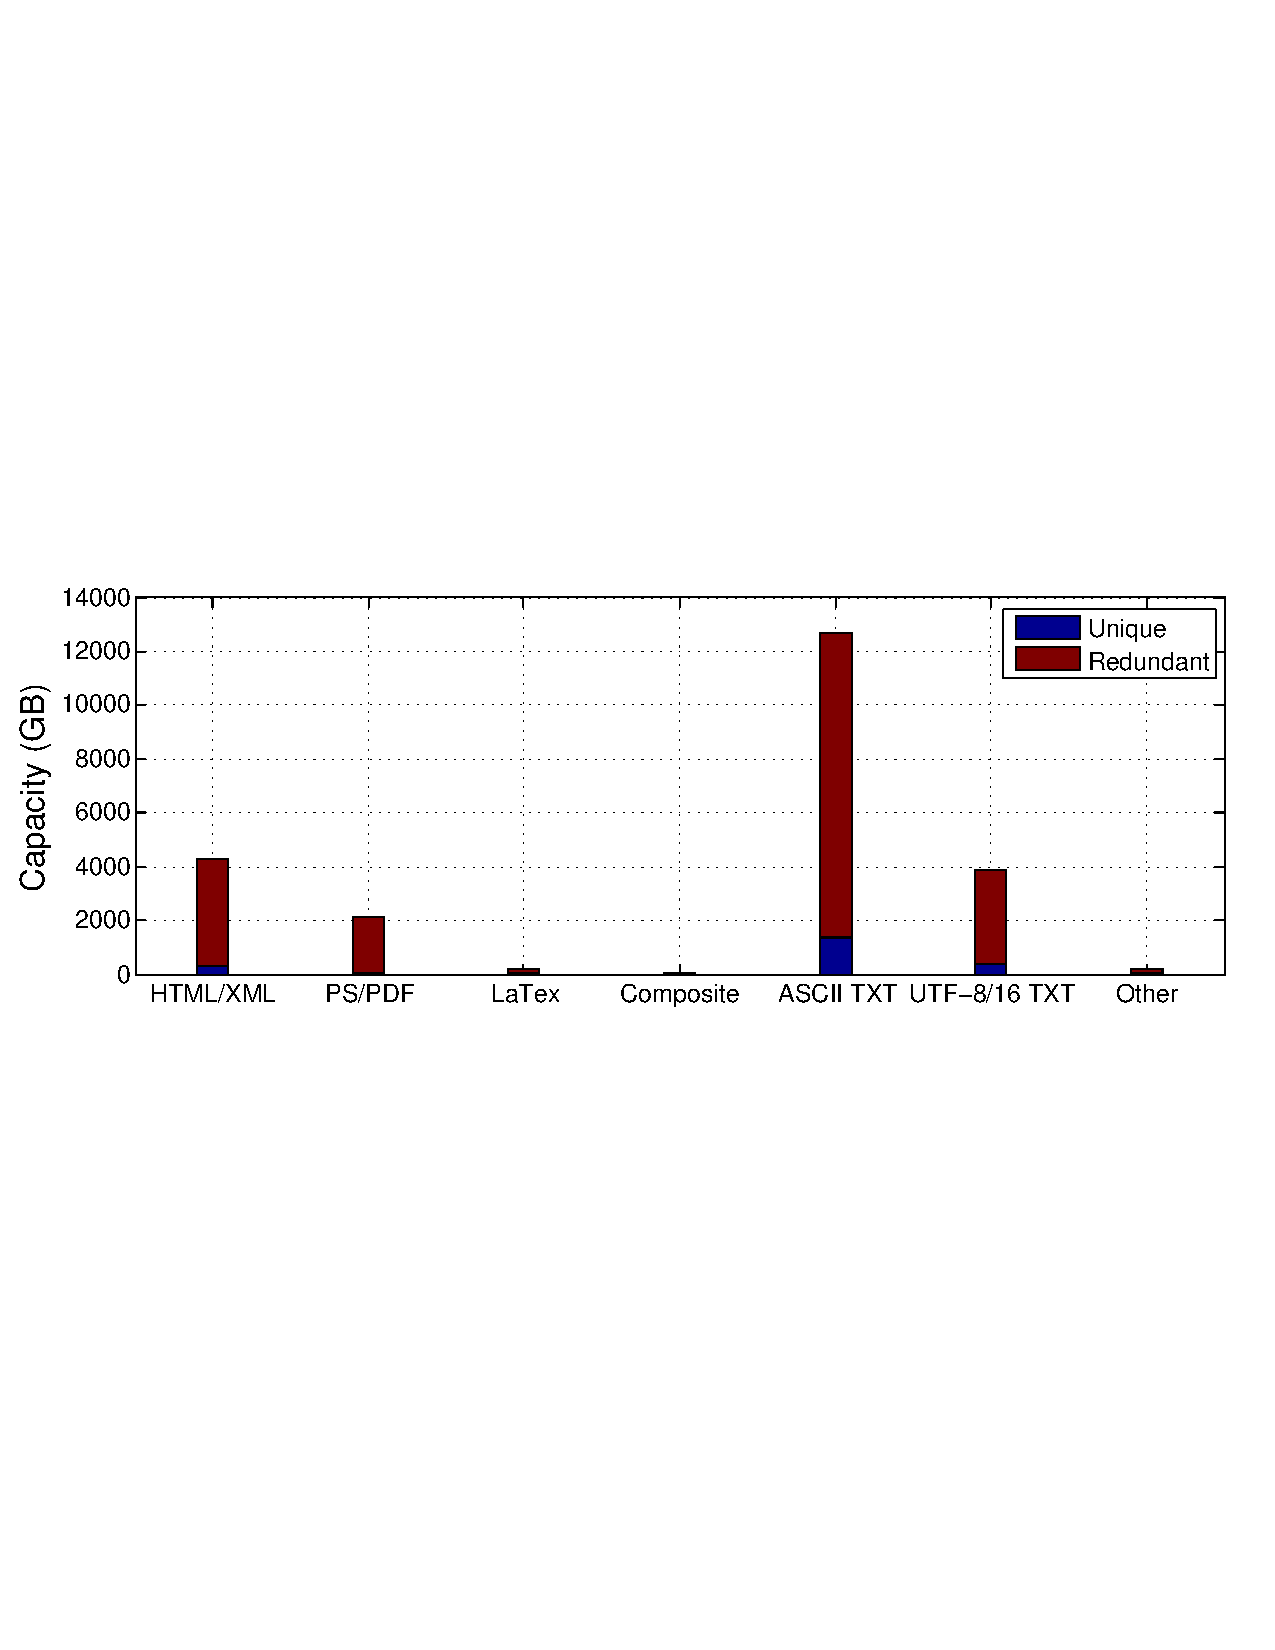
\includegraphics[width=0.5\textwidth]{graphs/type-utili-cap} %
%%\caption{Redundant data vs. unique data for documents.  %	} %
%%\label{fig:type-doc} %\end{figure}
%%
%%%https://pkgs.alpinelinux.org/contents?branch=edge&name=gnome-vfs-doc&arch=x86_64&repo=main
%%% presents redundant document distribution. We first group documents into two
%%categories: non-text documents and raw text documents.  %We see that ASCII
%%text files have the largest number of redundant document files (1,758,299,693,
%%79.7\%), which take up to 11TB storage space, indicating that users replicate
%%more ASCII text.  %12.4\% of the redundant documents are HTML/XML/XHTML
%%documents, which take up to 3.9 TB storage space, indicating users also
%%replicate HTML/XML/XHTML documents in images.  % %In addition to ASCII text,
%%5.2\% of redundant documents are UTF-8/16 unicode text, which take up 3.4 TB
%%storage space.  %Various documents are replicated in images, such as PS/PDF
%%documents (0.9\%), LaTex files (1.1\%) and Composite documents (0.01\%)
%%
%%%79.7\%, 5.2\%, and 12.4\% of redundant documents are ASCII text, UTF-8/16
%%text, and HTML/XML/XHTML, which take up over 11TB, 3.4TB, and 3.9TB redundant
%%storage, indicating that users replicate more ASCII text, UTF-8/16 text, and
%%HTML/XML/XHTML compare to other documents.  %type-utili-cap %type-script-cap
%%
%\paragraph{Databases (DB.)}
%%
%\begin{figure} 
%	\centering
%	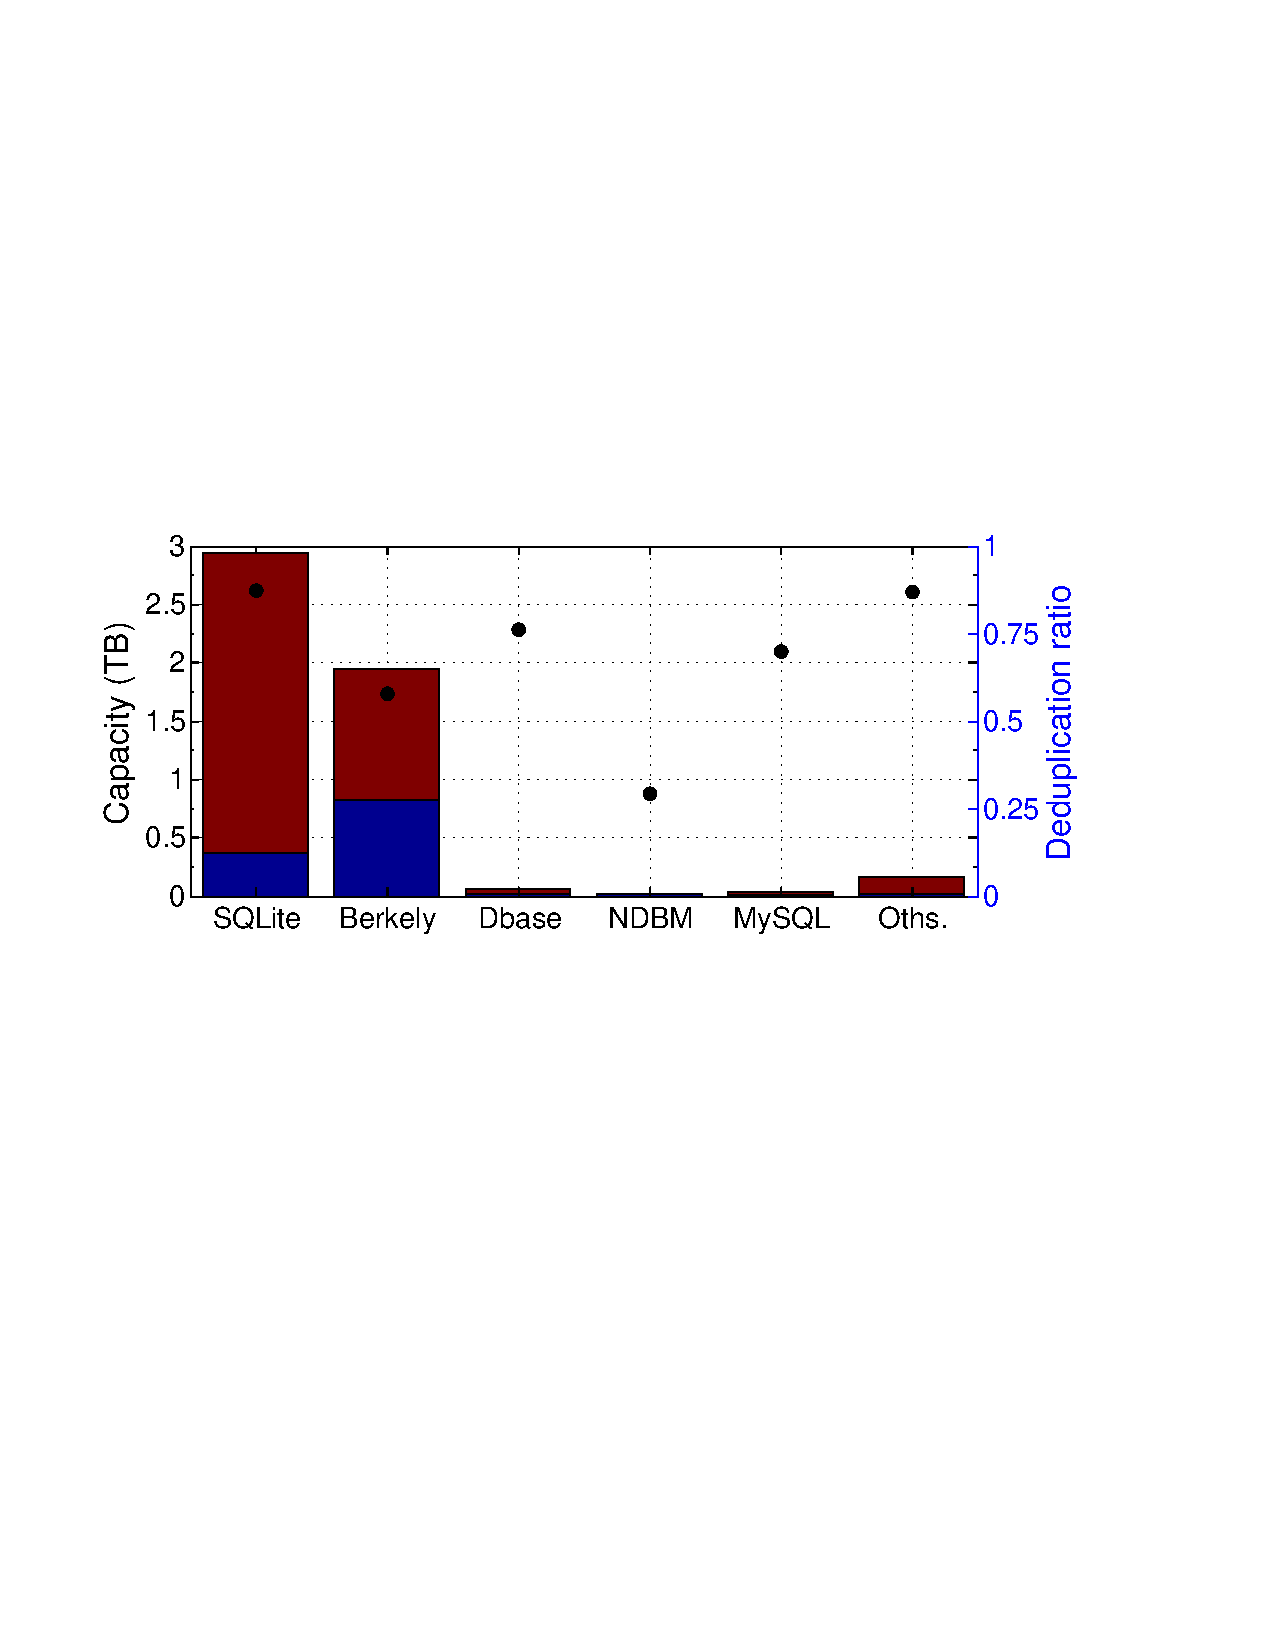
\includegraphics[width=0.4\textwidth]{graphs/dedup-db} \caption{Deduplication
%	results for database related files.  } 
%	\label{fig:dedup-db} 
%\end{figure}
%
%As discussed, Database related files have the lowest deduplication ratio at
%file-level. 
%%
%It makes sense because it's unusual for different users to create
%large amount of identical database files. 
%%
%Figure~\ref{fig:dedup-db} shows the
%deduplication ratio for different types of databases. 
%%
%We see that SQLite
%database files have the largest deduplication ratio of 87\% and could be
%deduplicated for saving up to half of the capacity. 
%%
%To find out why there are
%so many redundant SQLite files, we inspected SQLite files manually and found
%majority of redundant SQLite files are created by Yum~\cite{yum} for
%maintaining a list of well-know repositories.
%
%\textit{Finding 8: Databases have a low deduplication ratio. But SQLite files
%have the largest amount of redundant files and contribute a lot for saving
%capacity. The redundant SQLite files are mainly for saving identical list of
%repositories.}
%%
%%%primary_db.sqlite
%%
%%%Finding 4: 28.7\%, 30.9\%, and 11.9\% of redundant database files are
%%Berkeley DB, Mysql, and Dbase related files, which only take up over 1.1 TB,
%%26 GB, and 47.2 GB redundant storage, indicating that users replicate a lot
%%small database files related to Mysql and Berkeley DB. While there are only
%%7.3\% of SQLite files, which take up over 2.6TB storage space, indicating
%%SQLite files are much bigger than others.  % %Figure~\ref{fig:type-db}
%%presents database related redundant files. 30.9\% of redundant database
%%related files are related to MySQL, which only take up to 26GB storage space
%%while SQLite database related redundant files which only take up 7.3\% of
%%redundant database related files consume 2.56 TB storage space, indicating
%%users replicate more MySQL related files and bigger SQLite database related
%%files. %MySQL related files contains mysql table definitation files, mysql
%%misam index files, and mysql misam compressed data.  %Moreover, we also find
%%different redundant database related files are replicated in Docker images.
%%For example, 28.7\%, 11.86\%, and 5.57\% of redundant database files are
%%Berkeley DB, Dbase, and NDBM related files, which take up over 1.1 TB, 47.2
%%GB, and 7.7 GB redundant storage, indicating that users replicate database
%%files, especially, SQLite and Berkeley DB.  %While there are only 7.3\% of
%%SQLite files, which take up over 2.6TB storage space, indicating SQLite files
%%are much bigger than others.
%%
%%
%%%\begin{figure*}[t] %	\centering %	\begin{minipage}{0.35\textwidth} %
%%\centering %
%%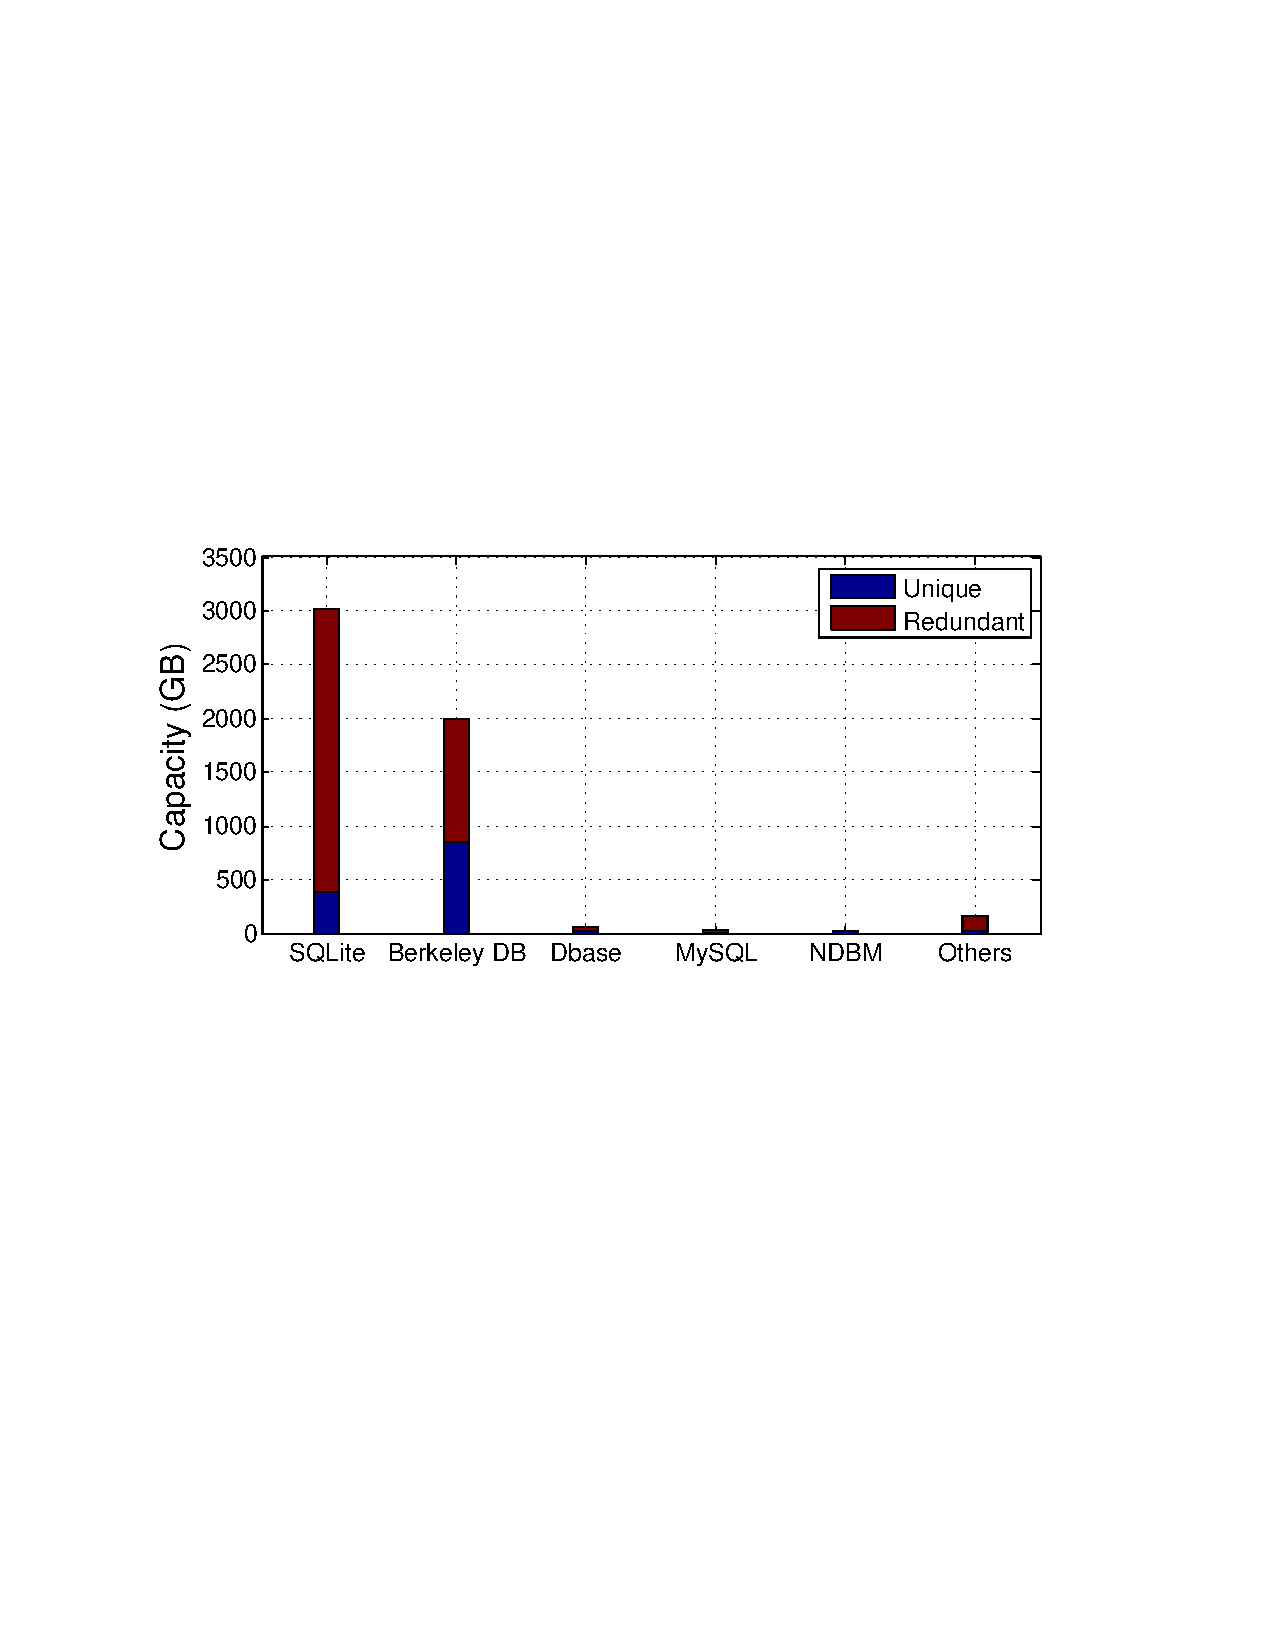
\includegraphics[width=1\textwidth]{graphs/type-db-cap.pdf} %
%%\caption{Redundant data vs. unique data for database related files} %
%%\label{fig:type-db} %	\end{minipage}% %
%%\begin{minipage}{0.278\textwidth} %		\centering %
%%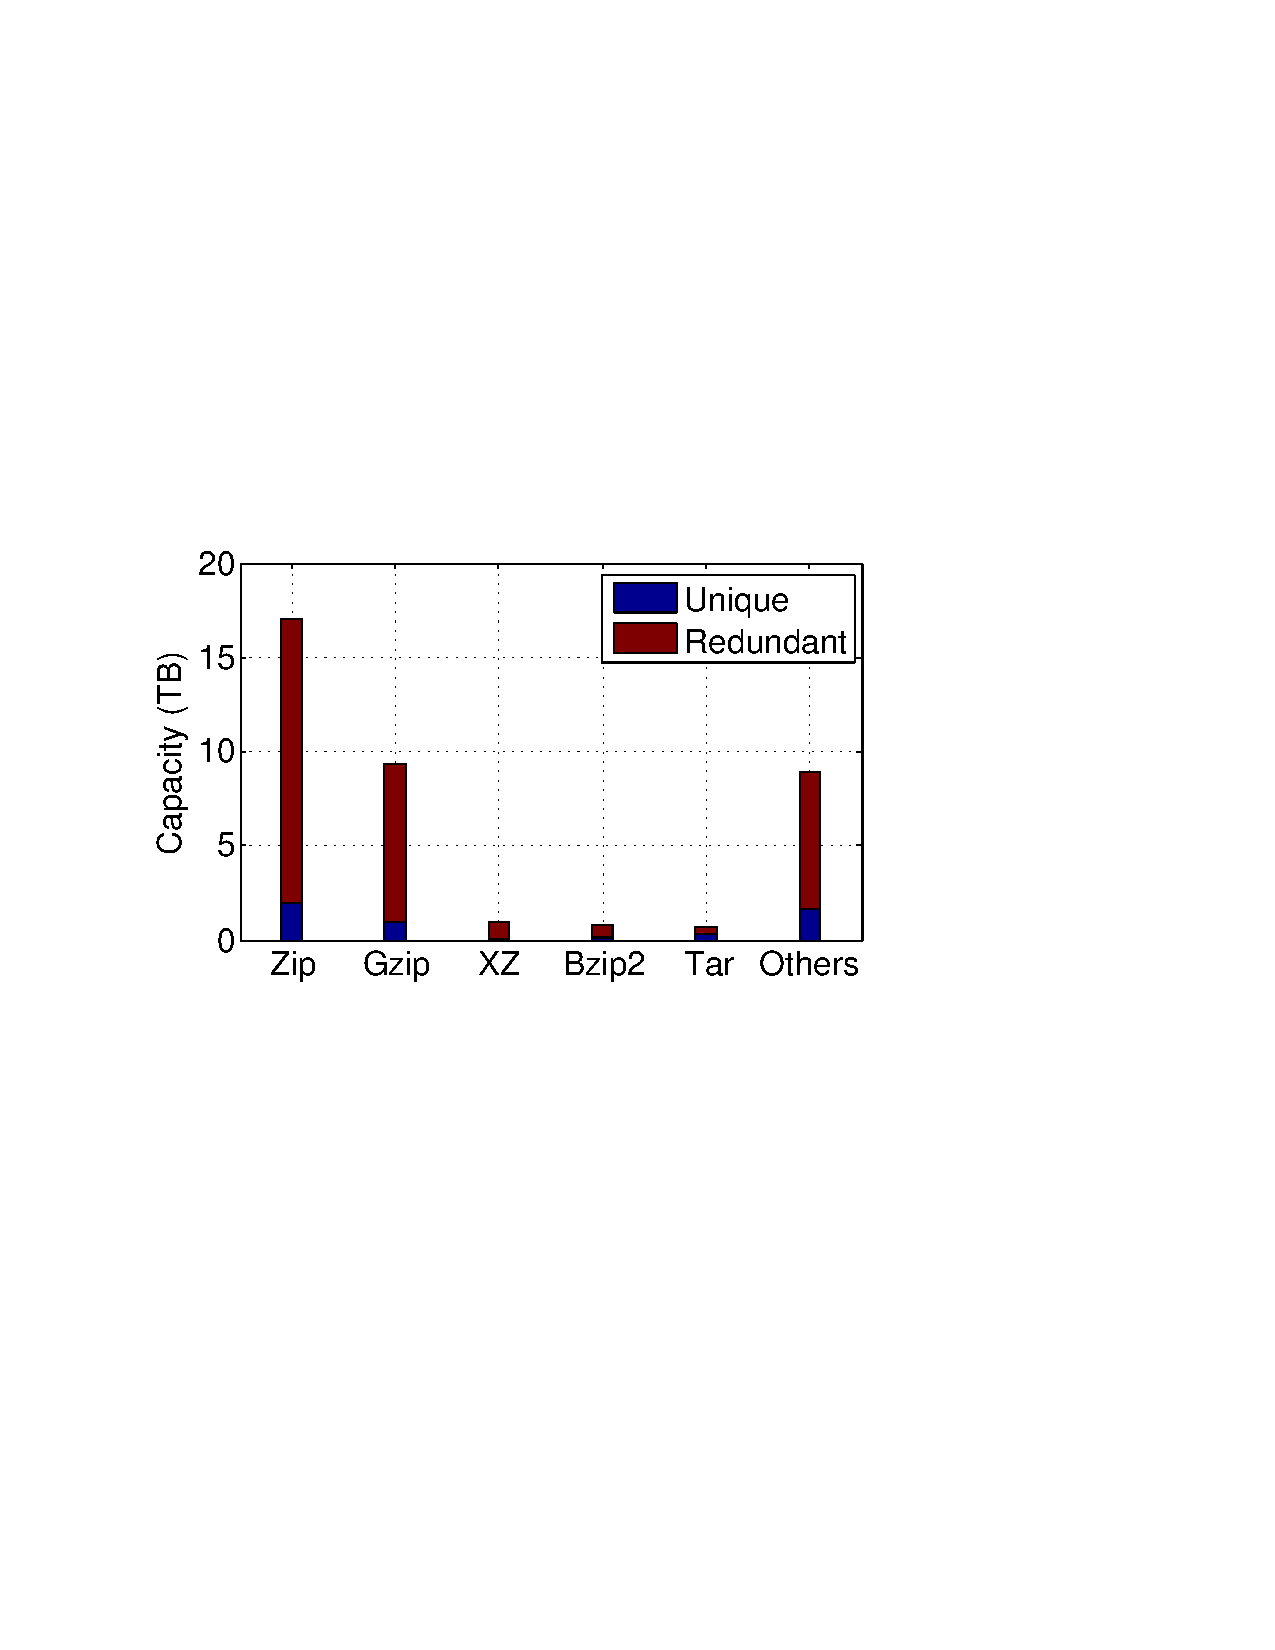
\includegraphics[width=1\textwidth]{graphs/type-tar-type} %
%%\caption{Redundant data vs. unique data for archival files} %
%%\label{fig:type-arch} %	\end{minipage} %
%%\begin{minipage}{0.28\textwidth} %		\centering %
%%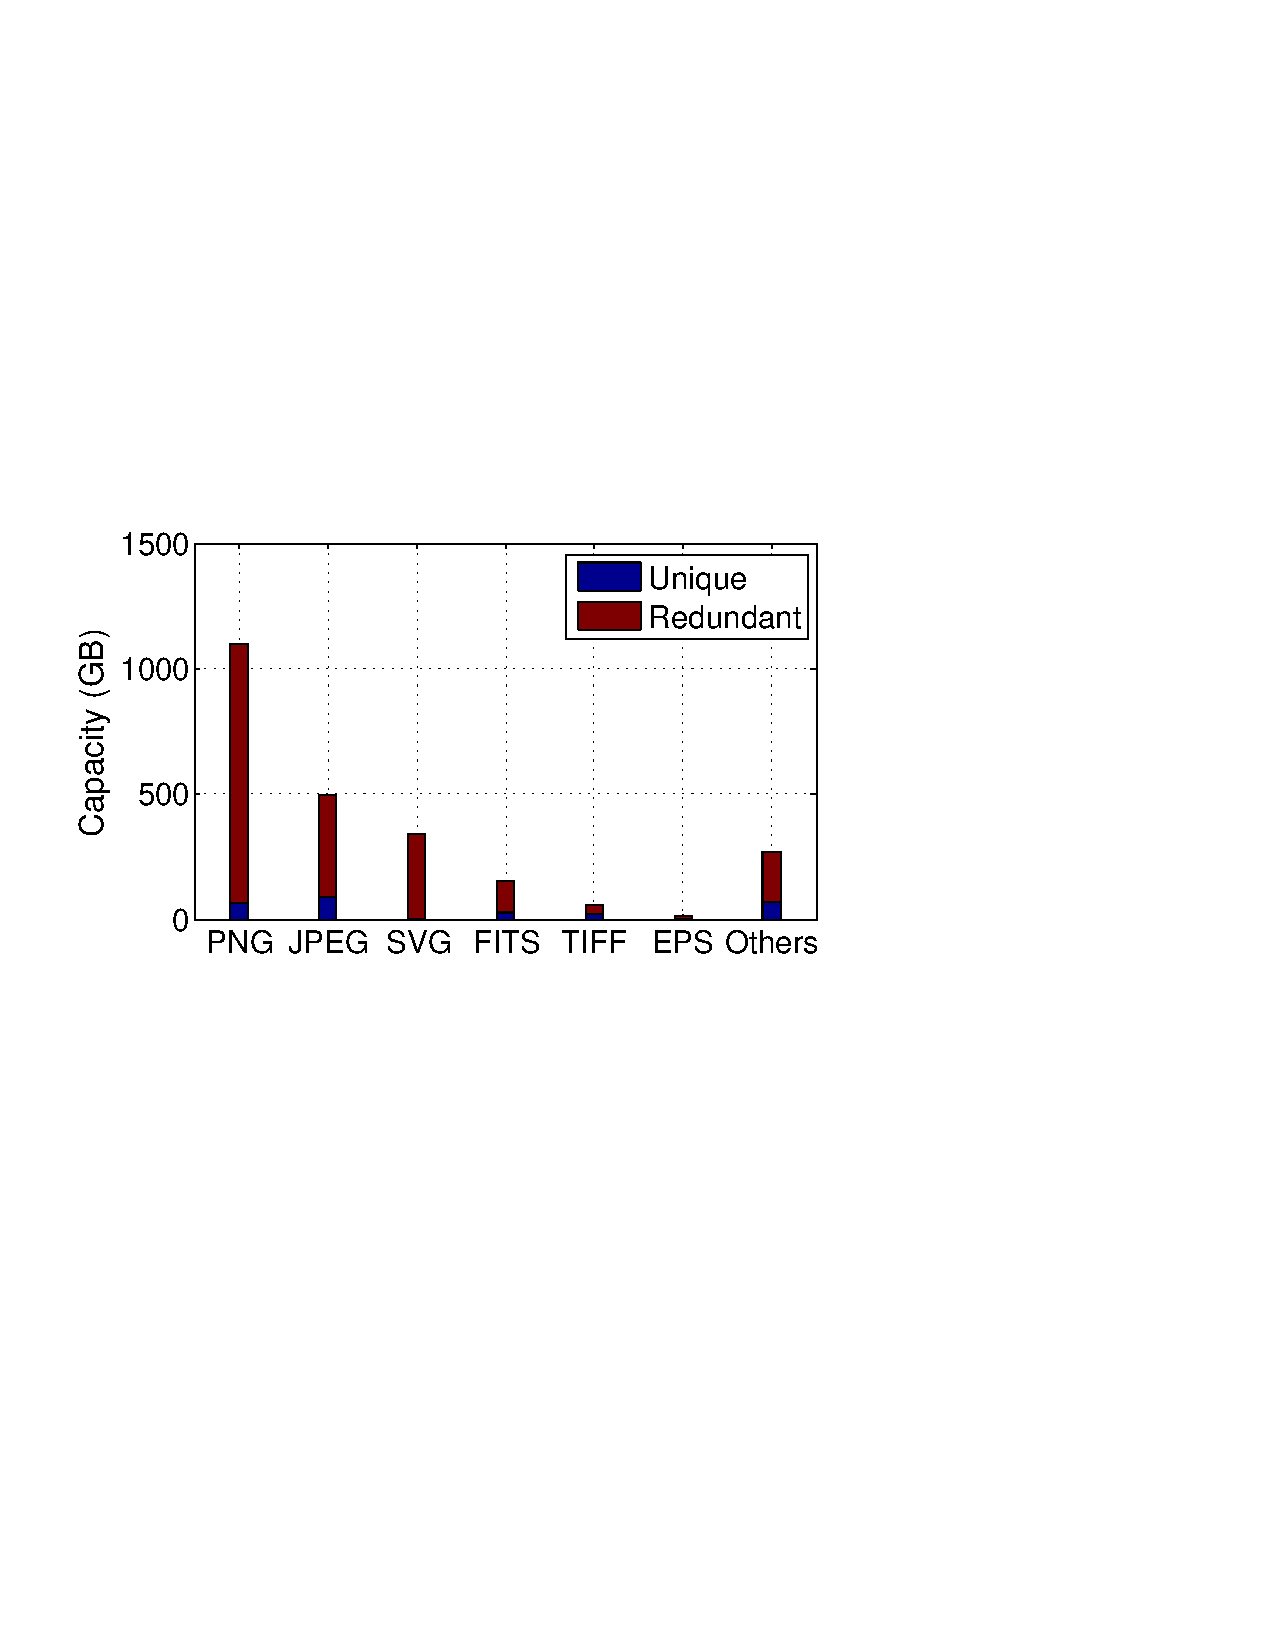
\includegraphics[width=1\textwidth]{graphs/type-image-cap} %
%%\caption{Redundant data vs. unique data for image files} %
%%\label{fig:type-img} %	\end{minipage} %\end{figure*}
%%
%%\paragraph{Archival (Arch.)}
%%
%%Figure~\ref{fig:type-arch} shows the deduplication ratio for each common
%%archival type.  We see that most of archival files have a high deduplication
%%over 80\% except tar archival files. Especially, Zip/Gzip files contribute to
%%most capacity savings after deduplication (62\%).  To understand why there are
%%so many redundant Zip/Gzip files, we manually inspected redundant Zip/Gzip
%%files and found that most of zip/Gzip files packages open source codes.  For
%%example, we found a redundant zip files called android-ndk-r12b.zip. It
%%packages the open source code--Android Native Development Kit (NDK)--that
%%allows Android application developers to include native code in their Android
%%application packages, compiled as JNI shared libraries~\cite{xxx}.
%%android-ndk-r12b.zip is available for downloading from GitHub. 
%%
%%\textit{Finding 9: Archival files have a high deduplication ratio. Majority of
%%Zip/Gzip files packages open source codes that are available online. We
%%suggest developers to remove the redundant archival files after unpacking to
%%reduce image size and save space.}
%%
%%%Finding 4: 89.5\% and 7.0\% of redundant archival files are Gzip files and
%%Zip files, which take up over 8.4 TB and 15.2 TB storage space, indicating
%%that users replicate more Gzip files and Zip files are much bigger than Gzip
%%files.  % % redundant archival file distribution. Gzip files have the largest
%%number of redundant archival files (89.5\%), which take up to 8TB storage
%%space, indicating that users replicate more Gzip compressed files. Although
%%Zip files only take 7.00\% of redundant archival files, they consume 15.5 TB
%%storage space since they are much bigger than Gzip files.  % %We found other
%%different kinds of archive files, such as XZ (0.42\%), Bzip2(0.96\%), and Tar
%%files(0.36\%).
%%
%\paragraph{Images (Img.)}
%
%\begin{figure} \centering
%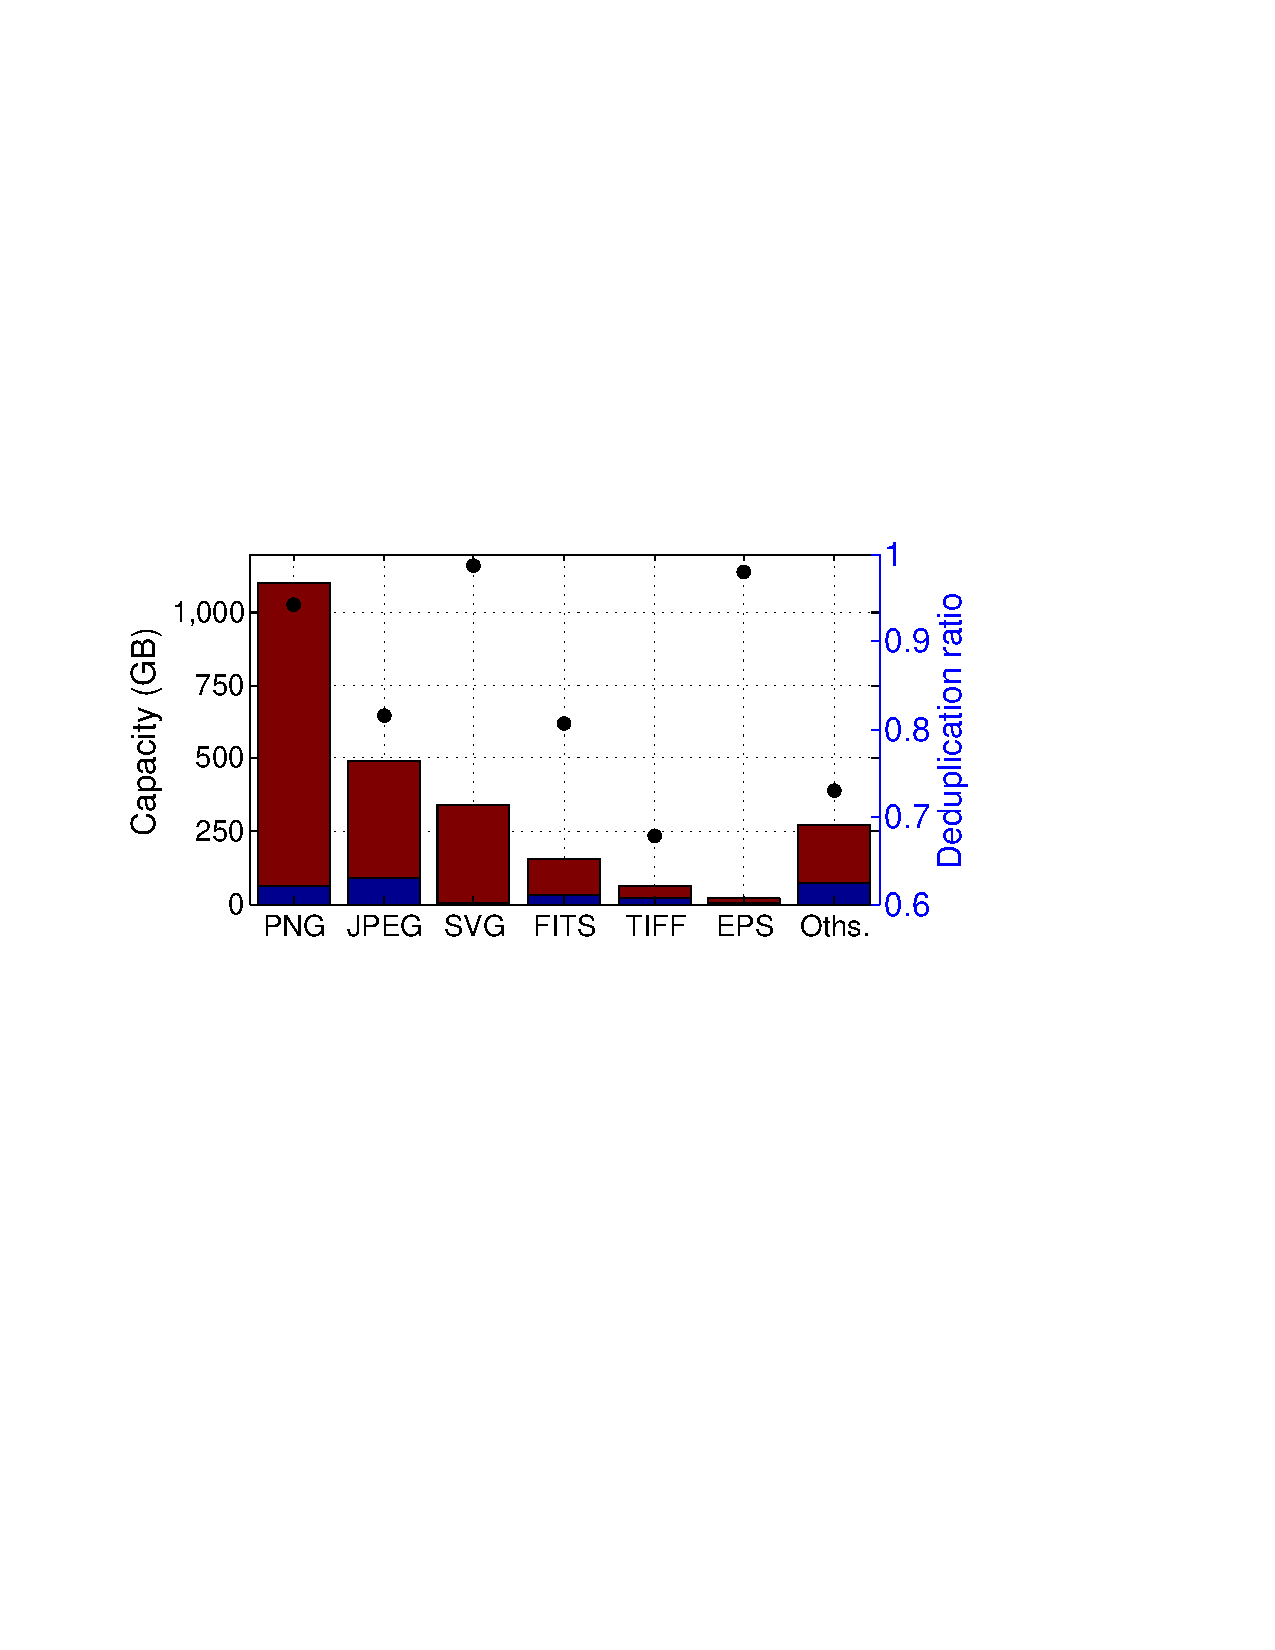
\includegraphics[width=0.35\textwidth]{graphs/dedup-img} \caption{Deduplication
%results for image files.  } \label{fig:dedup-img} \end{figure}
%
%Last, we present the redundant ratio for image files as shown in
%Figure~\ref{fig:dedup-img}.  We see that most of image files have a high
%deduplication ratio over 80\% except TIFF image files and TIFF image files.
%Especially, PNG images contributes to almost half of capacity savings after
%deduplication.  To understand why there are so many redundant image files, we
%inspected redundant PNG images and found plenty of PNG images are logo, icons,
%wallpapers, and images for testing.  For example, we found plenty of redundant
%PNG images related to matplotlib~\cite{matplotlib} for testing purpose. matplotlib is
%a Python 2D plotting library and available on GitHub.
%
%\textit{Finding 10: Most image files have a high deduplication ratio. PNG files
%contribute most to the space savings. Majority redundant PNG files are
%supplementary for documents or testing images for graphic editor softwares.}
%%%Finding 4: 67.8\%, 14.3\%, and 4.0\% of redundant image files are PNG, SVG,
%%and JPEG images, which take up over 1.01TB, 4.6 GB, and 401.5 GB storage
%%space, indicating that users also replicate image files, especially, PNG, SVG,
%%and JPEG files.  % % shows the redundant image file distribution. PNG image
%%files have the largest number of redundant image files (67.8\%), which take up
%%to over 1 TB storage space. 14.3\%, and 4.0\% of redundant image files are
%%SVG, and JPEG images, which take up over 4.6 GB and 401.5 GB storage space,
%%indicating that users also replicate image files, especially, PNG, SVG, and
%%JPEG files. Moreover, there are different redundant image file types, such as
%%FITS (0.05\%), TIFF (0.07\%), and EPS (0.01\%) image files.
%%
%%%\begin{figure} %	\centering %
%%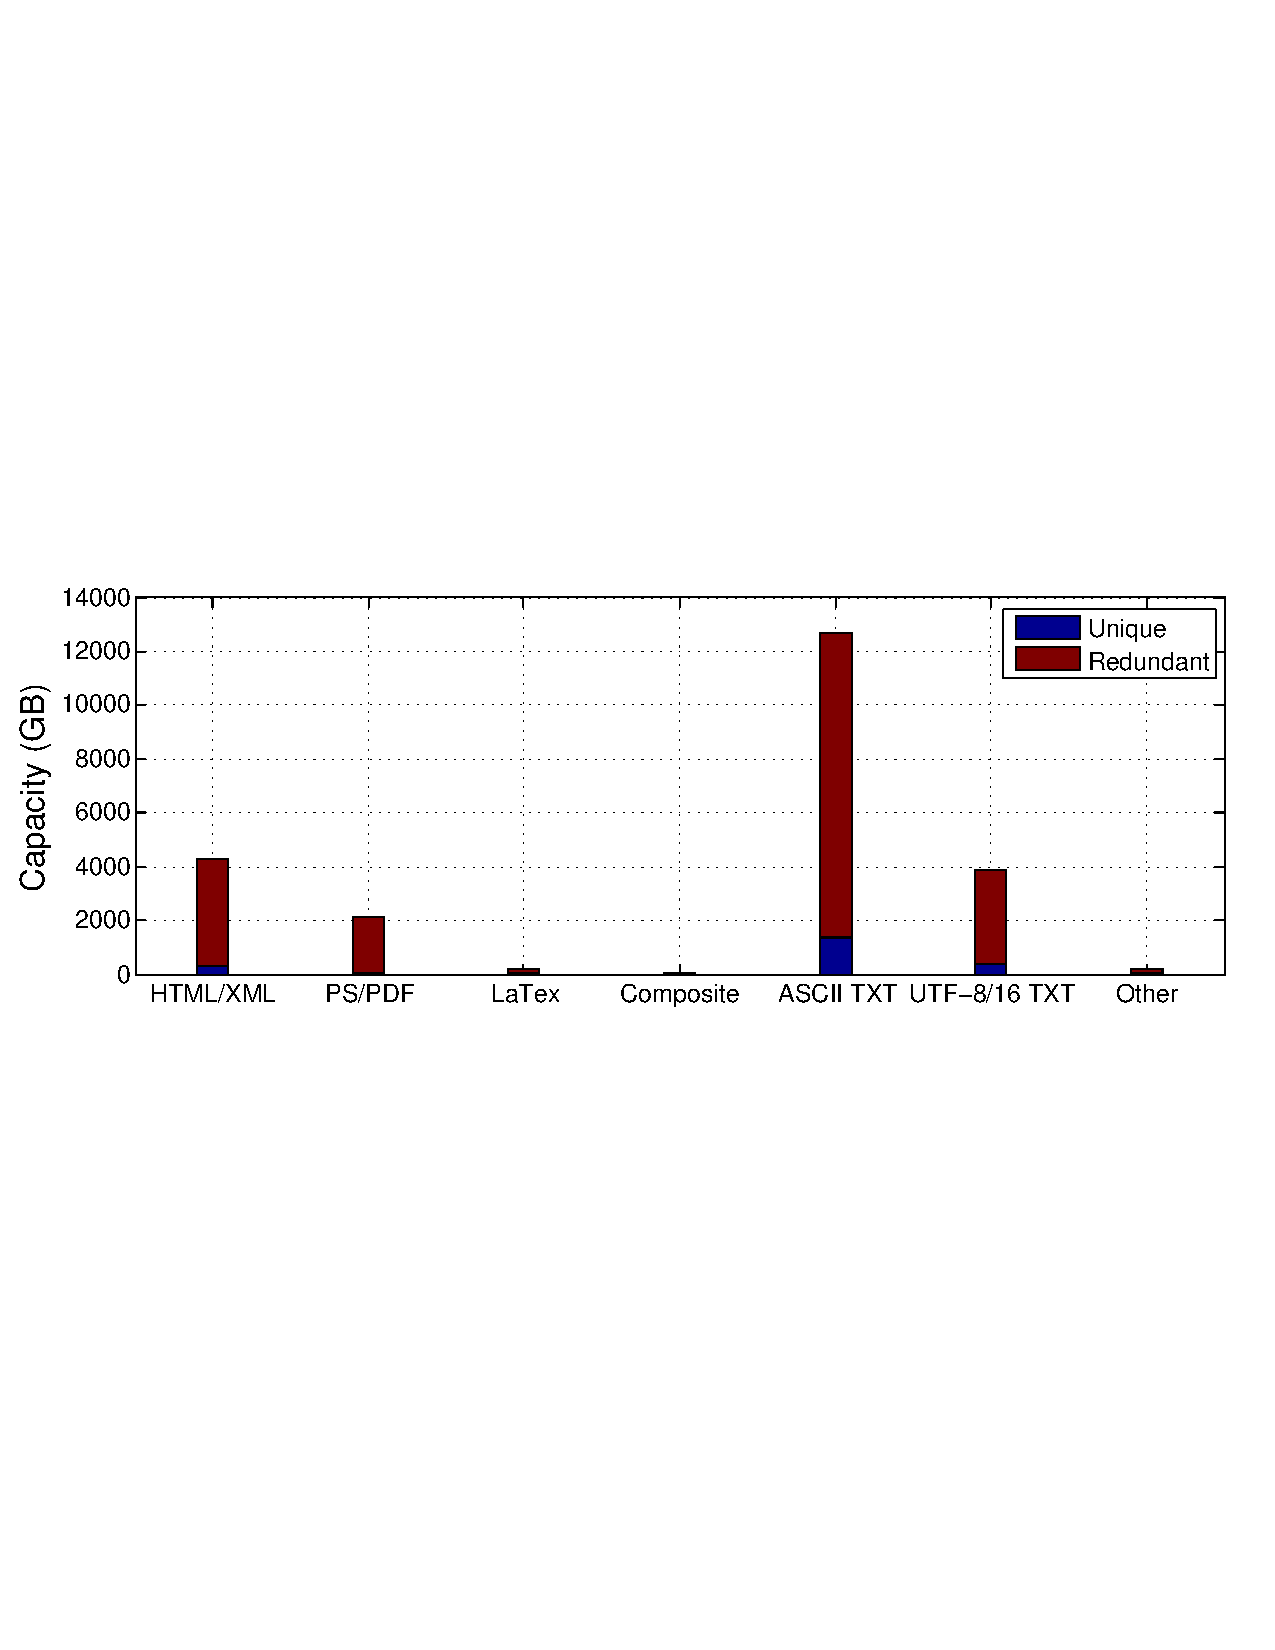
\includegraphics[width=0.35\textwidth]{graphs/type-utili-cap} %
%%\caption{Image file distribution.  %	} %	\label{fig:file_size}
%%%\end{figure}
%%
%%%======================================= %|             OLD VERSION
%%| %=======================================
%%
%%%\begin{table} %	\centering %	\scriptsize  %	\caption{Top 20
%%redundant files' characterization (sorted by repeat cnt.)} %
%%\label{tbl:top_dup_files_repeat_cnt} %
%%\begin{tabular}{|l|l|l|l|l|}%p{0.14\textwidth} %		\hline %
%%Filename & repeat cnt. & type & extension & size \\ %		\hline %
%%&   &   &   &  \\ %		\hline %		&   &   &   &   \\ %
%%\hline %		&   &   &  &    \\ %		\hline %
%%&  &  &  & \\ %		\hline %		& &  &   & \\ %
%%\hline %		& &  &   & \\ %		\hline %		&  &  &
%%& \\ %		\hline %	\end{tabular} %\end{table}
%%
%%%\begin{table} %	\centering %	\scriptsize  %	\caption{Top 20
%%redundant files' characterization (sorted by capacity)} %
%%\label{tbl:top_dup_files_cap} %
%%\begin{tabular}{|l|l|l|l|l|}%p{0.14\textwidth} %		\hline %
%%Filename & repeat cnt. & type & extension & size \\ %		\hline %
%%&   &   &   &  \\ %		\hline %		&   &   &   &   \\ %
%%\hline %		&   &   &  &    \\ %		\hline %
%%&  &  &  & \\ %		\hline %		& &  &   & \\ %
%%\hline %		& &  &   & \\ %		\hline %		&  &  &
%%& \\ %		\hline %	\end{tabular} %\end{table}
%%
%%
%%%\begin{table} %	\centering %	\scriptsize  %	\caption{Top redundant
%%file types} %	\label{tbl:top_dup_types} %
%%\begin{tabular}{|l|l|l|l|l|l|}%p{0.14\textwidth} %		\hline %
%%Type & extension & Num. & size & red. ratio (cnt.)  & red. ratio (cap.)\\ %
%%\hline %		&   &   &  & &   \\ %		\hline %
%%&   &   &  & &    \\ %		\hline %		&   &   &   & &   \\ %
%%\hline %		&  &  &  & & \\ %		\hline %
%%& &  &  & & \\ %		\hline %		& &  & & &  \\ %
%%\hline %		&  &  & & &  \\ %		\hline %
%%\end{tabular} %\end{table} 
%%
%%%\subsection{Redundant ratio for directories} % %\begin{table} %
%%\centering %	\scriptsize  %	%\begin{minipage}{.5\linewidth} %
%%\caption{Inter-dir redundant ratio for dirs in terms of file count and
%%capacity} \label{tbl:intra_dup_ratio_dirs} %
%%\begin{tabular}{|l|l|l|}%p{0.14\textwidth} %		\hline %
%%% after \\: \hline or \cline{col1-col2} \cline{col3-col4} ...  %
%%% after \\: \hline or \cline{col1-col2} \cline{col3-col4} ...  %
%%& File count & Capacity \\ %		\hline %		Avg. & 98.75\%
%%& 97.33\%\\ %		\hline %		Median & - & - \\ %
%%\hline %		Max. & 1 & 1\\ %		\hline %
%%Min.  & 0.87\%  & $<$ 0.00\%\\ %		\hline %		Stdev.
%%&  4.70\% & 10.49\\ %		\hline %		Layer dataset after
%%share.-dedup (Uncompressed) & -  & -\\ %		\hline %
%%Total layer dataset (Uncompressed) &  -	& -\\ %		\hline %
%%\end{tabular} %\end{table} % %\begin{table} %	\centering %	\scriptsize  %
%%%\begin{minipage}{.5\linewidth} %	\caption{Intra-dir redundant ratio for
%%dirs in terms of file count and capacity} \label{tbl:inter_dup_ratio_dirs} %
%%\begin{tabular}{|l|l|l|}%p{0.14\textwidth} %		\hline %
%%% after \\: \hline or \cline{col1-col2} \cline{col3-col4} ...  %
%%% after \\: \hline or \cline{col1-col2} \cline{col3-col4} ...  %
%%& File count & Capacity \\ %		\hline %		Avg. & 98.75\%
%%& 97.33\%\\ %		\hline %		Median & - & - \\ %
%%\hline %		Max. & 1 & 1\\ %		\hline %
%%Min.  & 0.87\%  & $<$ 0.00\%\\ %		\hline %		Stdev.
%%&  4.70\% & 10.49\\ %		\hline %		Layer dataset after
%%share.-dedup (Uncompressed) & -  & -\\ %		\hline %
%%Total layer dataset (Uncompressed) &  -	& -\\ %		\hline %
%%\end{tabular} %\end{table}
%%
%%%\subsection{Redundant directory characterization} % %\begin{table} %
%%\centering %	\scriptsize  %	%\begin{minipage}{.5\linewidth} %
%%\caption{Top redundant dirs'characterization} %
%%\label{tbl:top_dup_dirs} %	\begin{tabular}{|l|l|l|l|}%p{0.14\textwidth} %
%%\hline %		% after \\: \hline or \cline{col1-col2}
%%\cline{col3-col4} ...  %		% after \\: \hline or \cline{col1-col2}
%%\cline{col3-col4} ...  %		Name & Num. & Redundant ratio & Avg.
%%size \\ %		\hline %		home &   &   &     \\ %
%%\hline %		&   &   &      \\ %		\hline %
%%&   &   &      \\ %		\hline %		&  &  &  \\ %
%%\hline %		& &  &   \\ %		\hline %		& &  &
%%\\ %		\hline %		&  &  & \\ %		\hline %
%%\end{tabular} %\end{table} 
%%
%%%\begin{figure} %	\centering %
%%\includegraphics[width=0.5\textwidth]{graphs/} %	\caption{CDF of file
%%repeat count.  %	} %	\label{fig:file_repeat_count} %\end{figure}
%%
%%%\paragraph{Cumulative distribution and probability distribution of file size
%%in terms of unique file size, redundant file size, overall file size}
%%
%%
%%%\paragraph{Average file size by repeat count} % %There is no relation between
%%file repeat count and average file size.  % %\begin{figure} %	\centering %
%%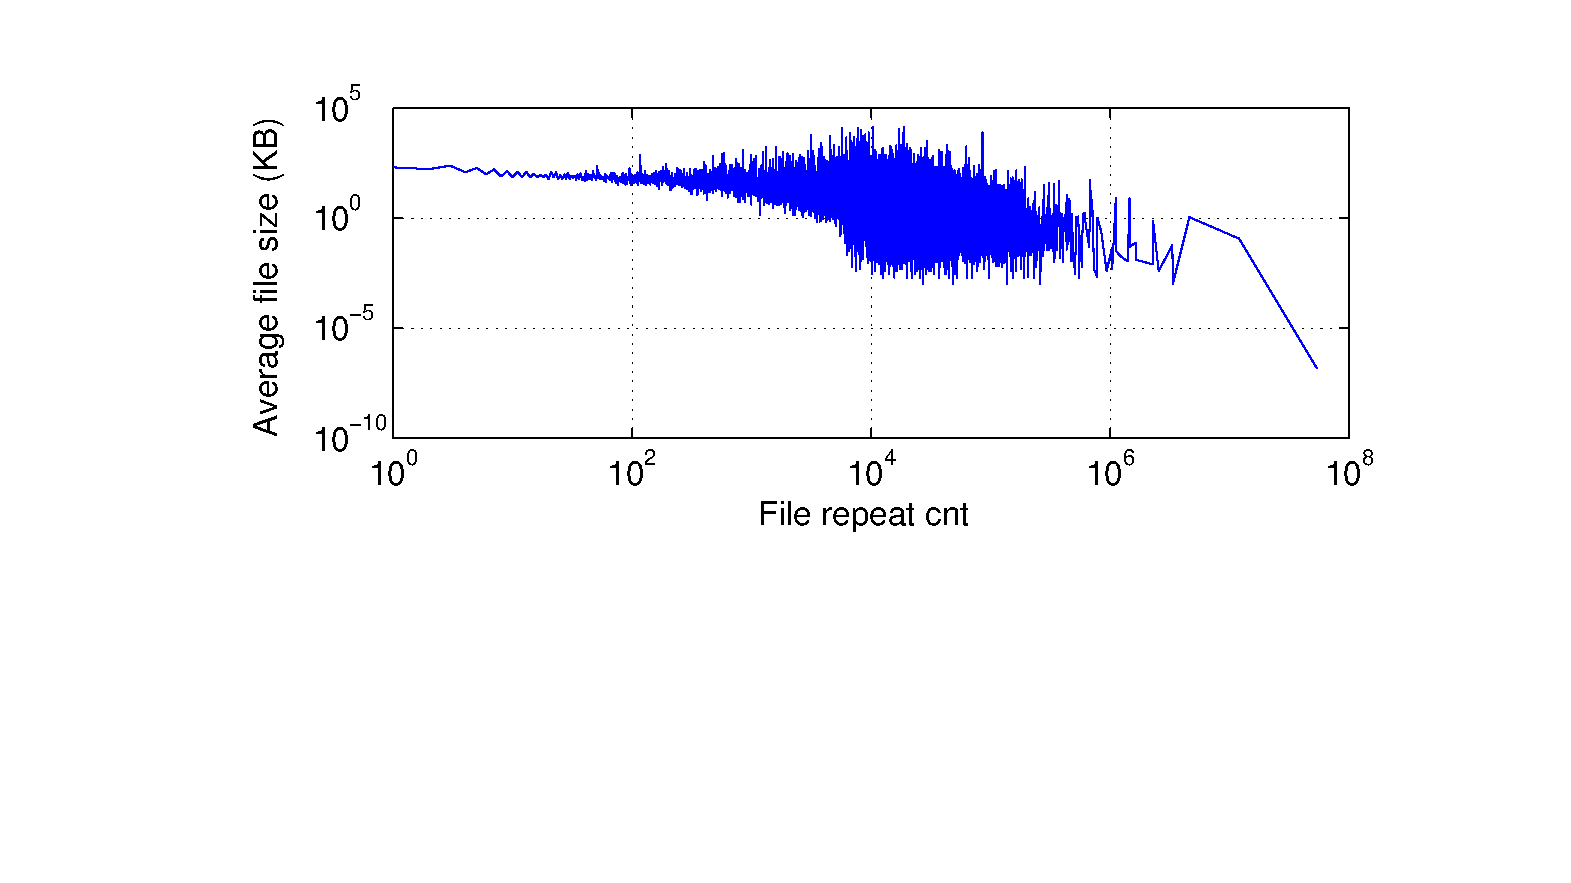
\includegraphics[width=0.5\textwidth]{graphs/avg_size_by_cnt.eps} %
%%\caption{Average file size with same repeat count.  %	} %
%%\label{fig_avg_size_by_cnt} %\end{figure} % %\paragraph{Redundant ratio by
%%file size for the files with the same content in terms of file count and
%%storage capacity} %Total size of redundant files with same content(TRS) %
%%%97\% of the TRSs are equal or less than 100MB.  % %\begin{figure} %
%%\centering %
%%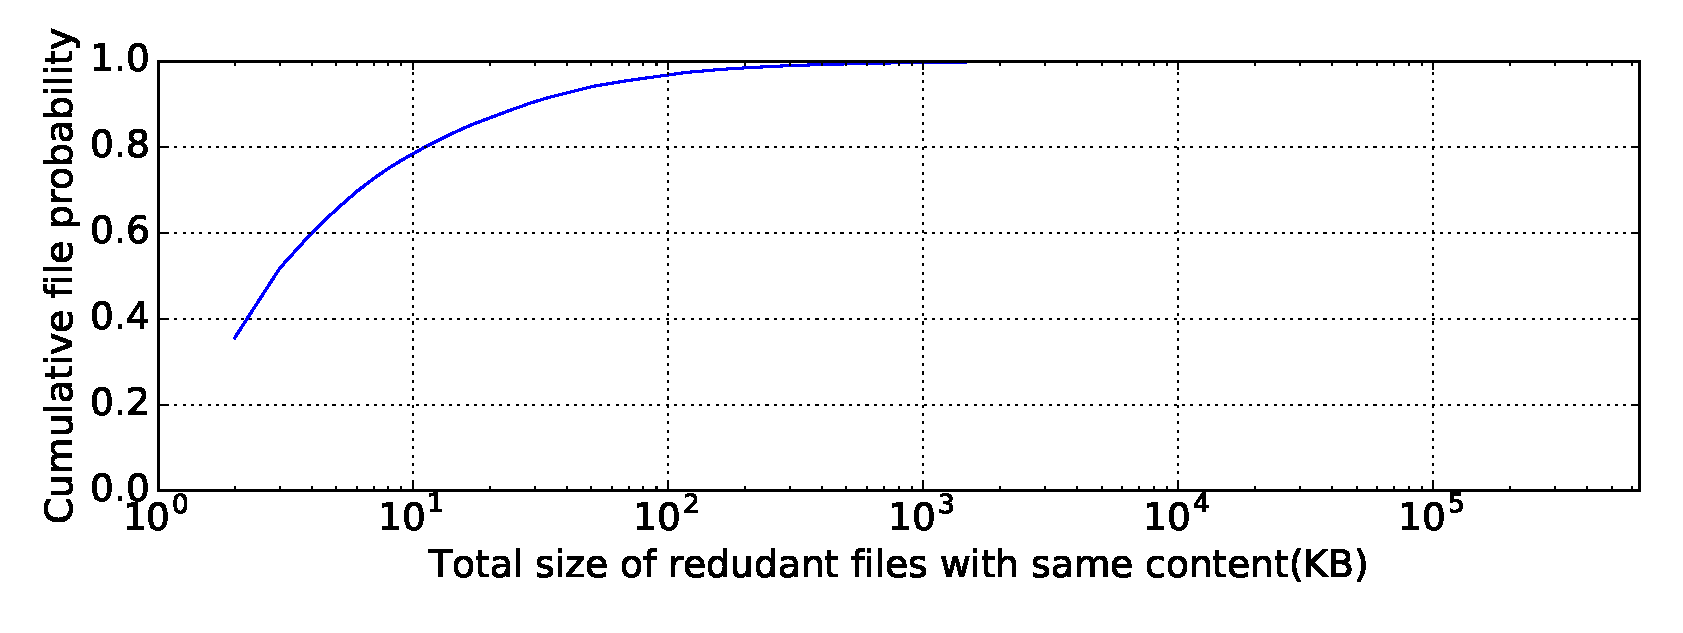
\includegraphics[width=0.5\textwidth]{graphs/Total_size_of_redudant_files_with_same_content-KB.eps}
%%%	\caption{CDF of total file size with same file content (MB).  %	} %
%%\label{fig_total_redundant_same_digest} %\end{figure} % %\paragraph{Redundant
%%ratio by repeat count for the files with the same repeat count in terms of
%%file count and storage capacity} % %However, with the increase of file repeat
%%count, the sum of file size with same repeat count becomes smaller.  %
%%%\begin{figure} %	\centering %
%%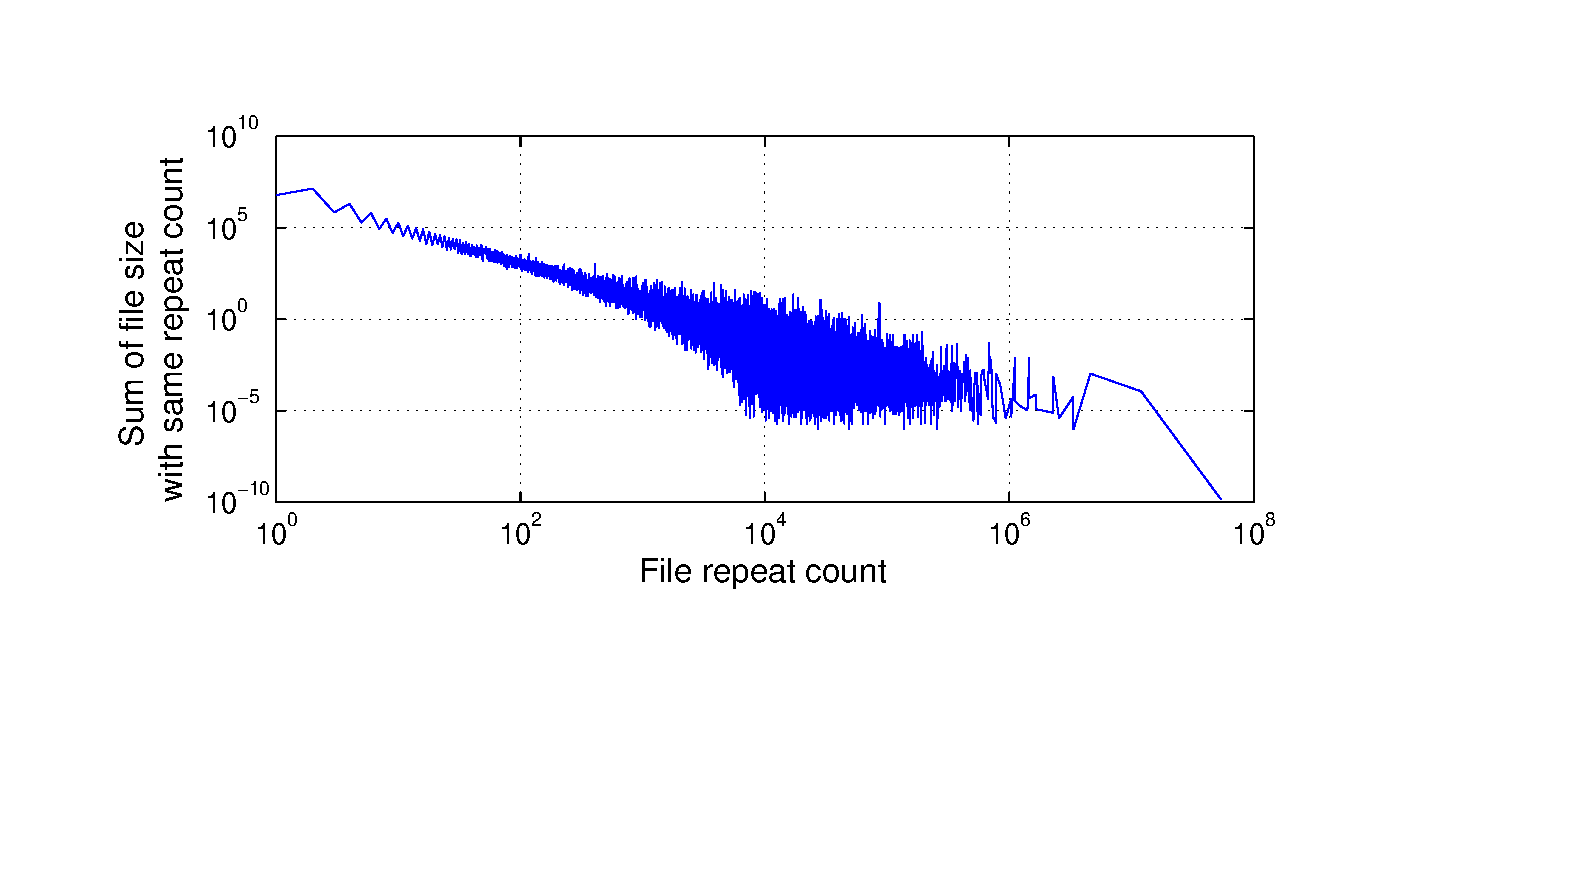
\includegraphics[width=0.5\textwidth]{graphs/sum_size_by_cnt.eps} %
%%\caption{Sum of file size with same repeat count.  %	} %
%%\label{fig_sum_by_cnt} %\end{figure}
%%
%%% %\paragraph{Cumulative distribution and probability distribution of file
%%repeat count} %\begin{table} %	\centering %	\scriptsize  %
%%%\begin{minipage}{.5\linewidth} %	\caption{Summary of image types}
%%\label{tbl:redundant_ratio} %	\begin{tabular}{|l|l|l|}%p{0.14\textwidth} %
%%\hline %		% after \\: \hline or \cline{col1-col2}
%%\cline{col3-col4} ...  %		% after \\: \hline or \cline{col1-col2}
%%\cline{col3-col4} ...  %		Image types & num. & avg. redundant
%%ratio  \\ %		\hline %		  &   &        \\ %
%%\hline %		  &   &         \\ %		\hline %
%%&   &       \\ %		   \hline %		other     &   &
%%\\ %		\hline %	\end{tabular} %\end{table}
%%
%%%\subsection{Redundant files with same filename and relative path} %
%%%\subsection{Common directories that contains redundant files} %
%%%\subsection{Redundant tar files} %\begin{table} %	\centering %
%%\scriptsize  %	%\begin{minipage}{.5\linewidth} %	\caption{Summary of
%%file \& dir. characterization} \label{tbl:sum_file_dir_char} %
%%\begin{tabular}{|l|l|l|l|l|}%p{0.14\textwidth} %		\hline %
%%% after \\: \hline or \cline{col1-col2} \cline{col3-col4} ...  %
%%% after \\: \hline or \cline{col1-col2} \cline{col3-col4} ...  %
%%Metrics & max & min & median & avg.\\ %		\hline %
%%File size &   &   &   &  \\ %		\hline %		File size
%%(repeat cnt. $>$ 1) &   &   &    &  \\ %		\hline %
%%File size (repeat cnt. $=$ 1) &   &   &    &  \\ %		\hline %
%%\hline %		Dir. size &  &  & & \\ %		\hline %
%%File cnt. per dir & &  &  & \\ %		\hline %
%%Redundant ratio & &  &  & \\ %		\hline %		Dir. depth  &
%%&  & & \\ %		\hline %	\end{tabular} %\end{table} 
